% Physics appendices of correlated_bias_prior_v2.tex, read with
% % Physics appendices of correlated_bias_prior_v2.tex, read with
% % Physics appendices of correlated_bias_prior_v2.tex, read with
% % Physics appendices of correlated_bias_prior_v2.tex, read with
% \input{appendix_physics} right after \appendix.  No preamble: the
% macros \ones, \Prec, \Cov and \T come from the main file.  The labels
% are shared with the mathematics appendices (appendix_math.tex).

\section{The models}
\label{sec:models}

This appendix first builds the prior without the tilt of
Eq.~\eqref{eq:summodel}: the kernel model, in which the exponential
kernel describes the whole deviation $\delta_i$ of a bin from its
group's trend.  Appendix~\ref{sec:memory} adds the free tilt, and the
kernel then describes the residual $\varepsilon_i$ around each group's
line.  In the appendices $b_i$ is the linear bias $b_{1,i}$ of bin $i$.

\subsection{Growth-tied, free, and correlated biases}
\label{sec:defs}

The growth-tied model sets $b_i = B_g/D(\bar{z}_i)$, with one free
amplitude $B_g$ per group.  The kernel model multiplies it by a
fractional deviation $\delta_i$,
\begin{align}
  b_i &\;=\; \frac{B_g}{D(\bar{z}_i)}\,\bigl(1 + \delta_i\bigr),
  \label{eq:model}
  \\
  \bigl\langle \delta_i\,\delta_j \bigr\rangle
  &\;=\; \sigma_g^2\,
  \exp\!\left(-\,\frac{|\bar{z}_i - \bar{z}_j|}{L}\right),
  \label{eq:priorkernel}
\end{align}
with $B_g$ still free (flat prior) and the prior zero across groups.
In the Fisher matrix the convenient parameters are the per-bin
amplitudes
\begin{equation}
  \beta_i \;\equiv\; B_g\,\bigl(1 + \delta_i\bigr),
  \qquad \text{fiducial } \beta_i = B_g,
  \label{eq:beta}
\end{equation}
so that $b_i = \beta_i / D(\bar{z}_i)$.  Since
$\beta_i - B_g = B_g\,\delta_i$, the prior covariance of the $\beta_i$
within one group is
\begin{equation}
  \Cov \;=\; \sigma_\beta^2\,\mathsf{R},
  \qquad
  \sigma_\beta \;=\; \sigma_g\,B_g,
  \qquad
  \mathsf{R}_{ij} \;=\; \exp\!\left(-\,\frac{|\bar{z}_i - \bar{z}_j|}{L}\right),
  \label{eq:covdef}
\end{equation}
with $\sigma_\beta$ the spread of one amplitude, in units of a bias, and
$\mathsf{R}$ the dimensionless correlation matrix.

\subsection{What $\sigma_g$ and $L$ mean}
\label{sec:jump}

The diagonal of the kernel gives the wander of a single bin,
$\mathrm{Var}(\delta_i) = \sigma_g^2$.  The correlation coefficient of
two bins at separation $\Delta z = |\bar{z}_i - \bar{z}_j|$ is
\begin{equation}
  r \;=\;
  \frac{\langle \delta_i \delta_j \rangle}
       {\sqrt{\langle \delta_i^2 \rangle\,\langle \delta_j^2 \rangle}}
  \;=\; e^{-\Delta z / L} ,
  \label{eq:rdef}
\end{equation}
set by the separation and $L$ alone.  The jump between the two bins has
variance
\begin{equation}
  \mathrm{Var}(\delta_i - \delta_j)
  \;=\;
  2\,\sigma_g^2\left(1 - e^{-\Delta z / L}\right)
  \;\approx\;
  \frac{2\,\sigma_g^2\,\Delta z}{L}
  \quad (\Delta z \ll L).
  \label{eq:jumpvar}
\end{equation}
At small separations the jump variance grows linearly with
$\Delta z$, as for a random walk; only beyond $L$ does the finite
wander pull the deviation back.  For neighbors at $\Delta z = 0.02$
with $L = 0.05$, $r = e^{-0.4} = 0.670$ and the exact rms jump is
$0.81\,\sigma_g$; the small-separation form gives $0.89\,\sigma_g$,
because $\Delta z/L = 0.4$ is not small.

\subsection{The free group amplitude and the projection}
\label{sec:projintro}

A plain Gaussian prior with covariance $\Cov$ would charge for moving
all $\beta_i$ of a group together, but that uniform shift is the free
amplitude $B_g$.  The repair removes the uniform direction: with
$\ones$ the ones vector of the group's $n$ bins, the prior precision
of a group's amplitudes is
\begin{equation}
  \Prec \;=\; \Cov^{-1}
  \;-\;
  \frac{\Cov^{-1}\ones\,\ones\T \Cov^{-1}}{\ones\T \Cov^{-1} \ones}.
  \label{eq:projdef}
\end{equation}
$\Prec\,\ones = 0$, so a uniform shift costs nothing; a pure shape
change keeps the penalty of the plain prior; $\Prec$ is positive
semidefinite (no displacement has a negative penalty) with rank
$n - 1$; and $\Prec$ is exactly the prior
obtained by sampling $B_g$ with a flat prior and marginalizing it.
Appendices~\ref{sec:twobins}, \ref{sec:threeviews} and
\ref{sec:general} show these for two bins, by marginalization, and for
$n$ bins.  Across groups the prior is zero, so the full prior
precision is block diagonal.

\section{Which $L$ and $\sigma_g$ are physical}
\label{sec:physical}

One case of bias evolution can be solved in closed form: a population
whose members are conserved.  This appendix derives it, measures its
deviation from the growth-tied trend, lists what breaks conservation in
a selected sample, and weighs the published measurements.

\subsection{A conserved population: the bias continuity equation}
\label{sec:conserved}

Take a sample whose membership never changes, with no velocity bias,
in linear theory.  The matter overdensity $\delta_m$ and the
galaxy-count overdensity $\delta_{\rm gal}$ then obey the same
continuity equation with the same velocity field, so the excess
clumping $\delta_{\rm gal} - \delta_m$ is frozen
(Appendix~\ref{app:continuity}).  With $b_c$ the linear bias at a
reference redshift $z_c$ and $\delta_m \propto D$, the frozen
difference gives~\cite{Fry1996}
\begin{equation}
  b(z) - 1
  \;=\;
  \bigl(b_c - 1\bigr)\,\frac{D(z_c)}{D(z)} :
  \label{eq:fry}
\end{equation}
the excess set at formation stays fixed while the matter clustering
grows, so the bias decays toward one.  The growth-tied shape freezes a
different quantity: constant $b\,D$ means a galaxy clustering amplitude
$b\,\delta_m$ that does not grow, which describes a selection that
picks, at each redshift, a different and rarer set of objects.

\subsection{The deviation from the growth-tied trend}
\label{sec:tilt}

Place the reference at a group's midpoint $z_c$, with
$b_c = B/D(z_c)$.  The ratio of Eq.~\eqref{eq:fry} to the growth-tied
bias $b_c\,D(z_c)/D(z)$ gives the deviation of Eq.~\eqref{eq:model},
\begin{equation}
  \delta(z)
  \;=\;
  \frac{D(z)/D(z_c) - 1}{b_c} ,
  \label{eq:tilt}
\end{equation}
zero at the midpoint, positive at lower redshift and negative at higher
redshift, and nearly linear across a group because $D$ is smooth.  In
flat $\Lambda$CDM with $\Omega_m = 0.3$ and the project's fiducial
amplitudes it is $+5.3\%$ and $-4.9\%$ at the ends of BGS ($B = 1.34$,
$0.1 < z < 0.4$, $b_c = 1.5$), $+2.4\%$ and $-2.2\%$ at the ends of LRG1
($B = 1.70$, $0.4 < z < 0.6$, $b_c = 2.2$), and $+2.6\%$ and $-2.3\%$ at
the ends of LRG3 ($B = 1.70$, $0.8 < z < 1.1$, $b_c = 2.7$).  Between
neighbors it changes by $0.3$--$0.7\%$ at $\Delta z = 0.02$ and
$0.8$--$1.7\%$ at $\Delta z = 0.05$: a smooth tilt, coherent over the
whole group.  For comparison, the neighbor rms of
Eq.~\eqref{eq:jumpvar} at $\Delta z = 0.02$ (and $0.05$) is $2.4\%$
($3.4\%$) for $\sigma_g = 3\%$ and $L = 0.05$, and $0.44\%$ ($0.67\%$)
for $\sigma_g = 1\%$ and $L = 0.2$.  Figure~\ref{fig:theorybz} draws
these shapes: the conserved curve is flatter than $B_g/D$ in every
group, while the BGS flux-limit curve is much steeper, and convex.

\begin{figure}[htbp]
  \centering
  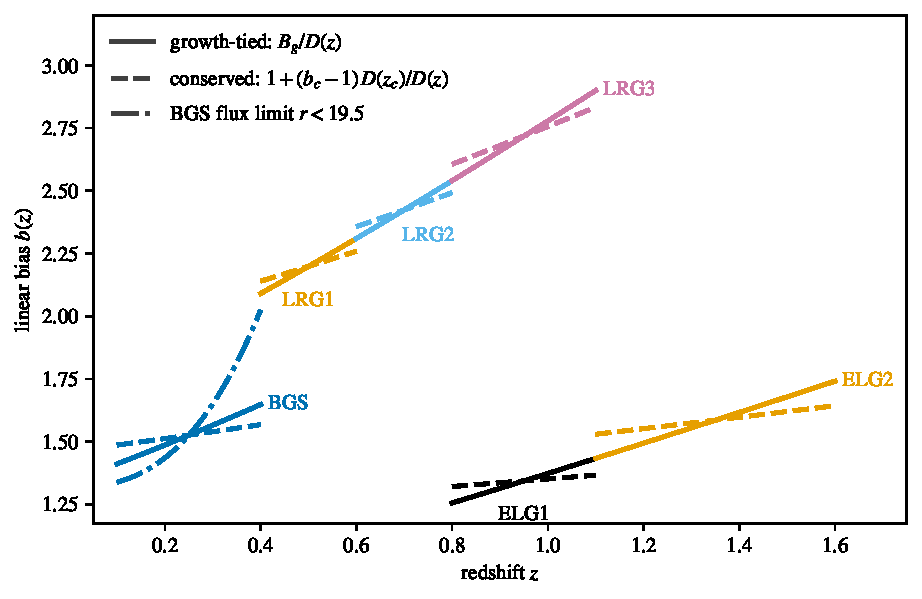
\includegraphics[width=\linewidth]{plots/theory_bz/theory_bz.pdf}
  \caption{The bias $b(z)$ of every group.  Solid: the growth-tied
    shape $B_g/D(z)$.  Dashed: a conserved population anchored at the
    group midpoint (Eq.~\eqref{eq:fry}).  Dash-dot, on BGS only: the
    $r < 19.5$ flux-limit bias, anchored at the same midpoint.}
  \label{fig:theorybz}
\end{figure}

\subsection{What breaks conservation in a selected sample}
\label{sec:selection}

\begin{itemize}
  \item \textbf{Threshold drift.}  A selection holds a roughly constant
    comoving density until the flux limit bites; beyond, it keeps only
    its brighter, more biased members.  The change is smooth, with $L$
    comparable to the group width.
  \item \textbf{Color-selection features.}  A spectral feature crossing
    a filter edge moves a color cut quickly in redshift.  The sharpest
    is the $4000$~\AA\ break, the step in an old galaxy's rest-frame
    spectrum at $4000$~\AA, which redshift slides across the filters: a
    filter edge $100$--$200$~\AA\ wide maps to
    $\Delta z = \Delta\lambda/(4000~\text{\AA}) \approx 0.03$--$0.05$.  The crossing is known; its
    amplitude in bias is unmeasured.
  \item \textbf{Mergers} turn two members into one.
  \item \textbf{Emission-line selection.}  An ELG belongs to the sample
    while its lines are strong, so membership follows the
    star-formation phase.
\end{itemize}

\subsection{What the measurements say}
\label{sec:evidence}

Each statement is tagged \emph{measured} (read from the cited source),
\emph{derived} (computed here from measured inputs) or \emph{assumed}.
Equation~\eqref{eq:fry} is from Fry~\cite{Fry1996};
Tegmark and Peebles~\cite{TegmarkPeebles1998} rederive it.

\paragraph{Massive red galaxies follow the conserved shape.}
SDSS and 2SLAQ LRGs at $0.19 < z < 0.55$, matched in color and
luminosity, show no significant evolution of the clustering amplitude
and merge at $7.5 \pm 2.3\%$ over that range, about $2.4\%$ per
Gyr~\cite{Wake2008} (measured).  The BOSS progenitors of the SDSS LRGs
merge at $2 \pm 1.5\%$ per Gyr and cluster as the continuity equation
predicts~\cite{Tojeiro2012}, and CMASS samples of fixed comoving
density at $0.43 < z < 0.7$ cluster like a conserved
population~\cite{Guo2013} (measured).  The bias of DESI-like LRGs in
photometric bins of $\Delta z \approx 0.1$ stays within $\pm 2.3\%$ of
$b = 1.5/D$ below $z = 0.83$, with the highest bin $6.4 \pm 6.4\%$
high~\cite{Zhou2021} (measured biases, residuals derived;
Figure~\ref{fig:zhou}).

\begin{figure}[htbp]
  \centering
  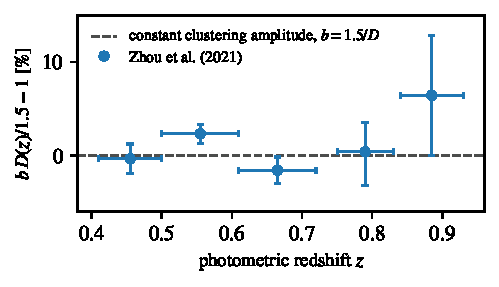
\includegraphics{plots/zhou_lrg_bias/zhou_lrg_bias.pdf}
  \caption{The measured bias of DESI-like LRGs~\cite{Zhou2021} as a
    fractional residual around $b = 1.5/D$, with $D$ at each
    photometric bin's center (flat $\Lambda$CDM, $\Omega_m = 0.3$);
    horizontal bars: the bin edges.}
  \label{fig:zhou}
\end{figure}

\paragraph{The selections drift.}
The DESI LRG cuts hold the comoving density near
$5 \times 10^{-4}\,(h/{\rm Mpc})^3$ at $0.4 < z < 0.8$ and hand over to
a fixed flux limit beyond~\cite{Zhou2023lrg} (measured).  That limit
raises the luminosity threshold by $0.27$ magnitudes per
$\Delta z = 0.1$ at $z \approx 1$; times the threshold-bias slope of
SDSS luminosity-threshold samples, $b\,(\sigma_8/0.8) = 1.06 +
0.21\,(L_{\rm th}/L_*)^{1.12}$~\cite{Zehavi2011} ($0.5$--$1.0$ in bias
per magnitude near LRG luminosities; measured), it drifts the LRG3 bias
by $6$--$11\%$ per $\Delta z = 0.1$ on top of $B/D$ (derived, from an
$r$-band relation outside its calibrated range, so only the direction
and order of magnitude hold).  BGS Bright is magnitude limited at
$r < 19.5$~\cite{Hahn2023} (measured), which drives a $10$--$25\%$ bias
drift across the group (derived; Appendix~\ref{app:bgsflux}).

\paragraph{The ELG bias shape is stable.}
Fits of the halo occupation distribution (HOD: how many sample
galaxies live in a halo of each mass) to the DESI One-Percent ELGs in
$0.8 < z < 1.1$ and
$1.1 < z < 1.6$ agree within one sigma~\cite{Rocher2023} (measured);
at these host masses the halo bias depends weakly on mass, so the
implied drift is at the percent level (derived, slope assumed).  The
[OII] doublet loses signal-to-noise in windows
$\Delta z \approx 0.001$--$0.01$ wide where it lands on sky lines,
especially at $z > 1.5$~\cite{Raichoor2023} (measured): the one
short-separation mechanism with a measured location, with an assumed
bias amplitude of $1$--$2\%$.

\paragraph{Nothing resolves bias below $\Delta z \approx 0.1$.}
The CMB-lensing tomography of the same samples~\cite{White2022,
Sailer2024, Sailer2025}, on the photometric samples of
Zhou et al.~\cite{Zhou2023tomo}, uses bins of about $0.15$ with one
free bias per bin and finds smooth models that fit.  Below
$\Delta z \approx 0.1$ this note rests on the continuity equation and
the selection arguments.

\section{The memory model}
\label{sec:memory}

\subsection{Why a second model}
\label{sec:memwhy}

Every deviation above except the sky-line windows is a monotonic drift:
the conserved-population tilt (about $1\%$ per $\Delta z = 0.05$), the
LRG3 magnitude-limit drift ($6$--$11\%$ per $\Delta z = 0.1$) and the
BGS flux-limit drift ($10$--$25\%$ across the group).  The kernel model
admits such a drift only at a price: to pass a $20\%$ drift with
$L \leq 0.1$ it takes $\sigma_g = 10$--$15\%$, which also allows about
$10\%$ scatter between neighbors that no identified mechanism
produces.  One $\sigma_g$ controls both, so the kernel cannot say
``large smooth drift, small local scatter''.  The memory model
separates the two.

\subsection{Why the kernel forgets}
\label{sec:memforget}

At $L = 0.05$, bins $0.15$ apart share $e^{-3} \approx 0.05$ of their
deviation.  With $r_k = e^{-(\bar{z}_{k+1} - \bar{z}_k)/L}$ the
correlation of neighbors $k$ and $k+1$, the best guess of the next bin
given all earlier ones is (Appendix~\ref{app:chain})
\begin{equation}
  \mathrm{E}\bigl[\delta_{k+1} \mid \delta_1, \dots, \delta_k\bigr]
  \;=\; r_k\, \delta_k :
  \label{eq:memmarkov}
\end{equation}
only the nearest neighbor matters, and the influence of any one bin
fades along the chain.

\subsection{The model, and why it remembers}
\label{sec:memmodel}

The memory model adds a tilt per group and splits the deviation into a
line and a residual,
\begin{equation}
  \delta_i \;=\; s_g\, v_i + \varepsilon_i,
  \qquad
  v_i \;=\; \bar{z}_i - \bar{z}_g,
  \label{eq:memdef}
\end{equation}
with $s_g$ a free tilt (flat prior, like $B_g$) and $\varepsilon_i$
carrying the kernel of Eq.~\eqref{eq:priorkernel}: the model of
Eqs.~\eqref{eq:summodel} and \eqref{eq:sumkernel}.  Giving the slope a
Gaussian prior of variance $\tau^2$ first (the flat prior is
$\tau \to \infty$), the deviations have covariance
\begin{equation}
  \mathrm{Cov}(\delta_i, \delta_j)
  \;=\;
  \tau^2\, v_i\, v_j
  \;+\;
  \sigma_g^2\, e^{-|\bar{z}_i - \bar{z}_j|/L} .
  \label{eq:memcov}
\end{equation}
The new term does not decay with separation.  Far beyond $L$ the
correlation coefficient tends to
\begin{equation}
  \rho_{ij}
  \;\longrightarrow\;
  \frac{\tau^2 v_i v_j}
       {\sqrt{\bigl(\tau^2 v_i^2 + \sigma_g^2\bigr)
              \bigl(\tau^2 v_j^2 + \sigma_g^2\bigr)}}
  \;\longrightarrow\; \pm 1
  \quad \text{when } \tau |v| \gg \sigma_g :
  \label{eq:memrho}
\end{equation}
the two ends of a group remember each other through the shared slope.
The best guess of the next bin becomes
\begin{equation}
  \mathrm{E}\bigl[\delta_{k+1} \mid \delta_1, \dots, \delta_k\bigr]
  \;=\;
  \hat{c} + \hat{s}_g\, v_{k+1}
  \;+\;
  r_k\,\bigl(\delta_k - \hat{c} - \hat{s}_g\, v_k\bigr),
  \label{eq:memkriging}
\end{equation}
with $(\hat{c}, \hat{s}_g)$ the level and slope of the best straight
line through all past bins, weighted by $\Cov^{-1}$: every past bin
enters through the fitted line, and only the wiggle around it stays
Markov (the universal-kriging predictor; kriging is the geostatistics
name for the best linear prediction from correlated data;
Appendix~\ref{app:memory}).
Figure~\ref{fig:theorydraws} shows the difference on the BGS bins at
$\Delta z = 0.02$: kernel draws wide enough to admit the BGS drift
zigzag and forget, while memory draws are lines with small wiggles,
among which the drift looks typical.

\begin{figure}[htbp]
  \centering
  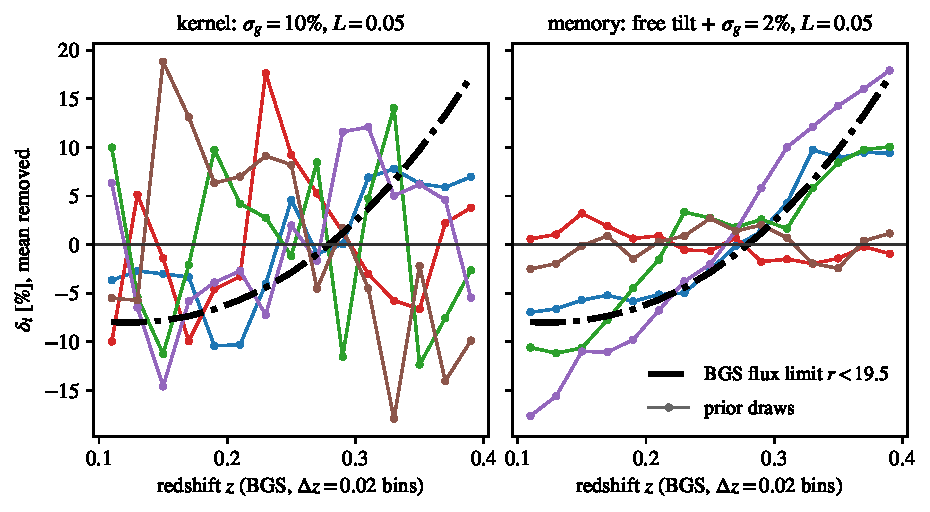
\includegraphics[width=\linewidth]{plots/theory_draws/theory_draws.pdf}
  \caption{Random prior draws of the deviations of the 15 BGS bins at
    $\Delta z = 0.02$, each draw's mean removed ($B_g$ is free).  Thick
    dash-dot: the BGS flux-limit drift.  Left: the kernel model.
    Right: the memory model, whose tilt is free in the model and drawn
    here, for display only, from a Gaussian of width $0.6$ per unit
    redshift.}
  \label{fig:theorydraws}
\end{figure}

\subsection{Why the memory model differs physically}
\label{sec:memphysics}

A selected sample changes along a group in two ways.  Coherent changes
move every bin the same way: a threshold that rises with distance, the
debiasing of a conserved population.  Local changes move bins
independently and are forgotten over a short range: the sky-line
windows and filter-edge crossings of Appendix~\ref{sec:selection}.  The
memory model gives the first kind to the tilt and the second to the
kernel.  One line suffices for the coherent kind, because the drifts
are smooth functions of $D(z)$ and the distance modulus.  The best
equal-weight line through each group's conserved deviation at the
$\Delta z = 0.05$ bin centers (derived; amplitudes $1.34$ for BGS,
$1.70$ for the LRGs and $0.84$ for the ELGs) removes deviations that
span $3$--$11\%$ and leaves $0.02$--$0.16\%$ rms, at most $0.27\%$
(ELG2).  The BGS flux-limit drift is larger and convex: it spans
$22.3\%$, and its best line leaves $2.4\%$ rms and $3.3\%$ at most
(Appendix~\ref{app:bgsflux}).  Figure~\ref{fig:theorydelta} shows both.
In the memory model $\sigma_g$ is the departure from the group's own
line, curvature plus local scatter: about $0.1\%$ for a conserved
population, $1$--$2\%$ for local selection features, $2$--$3\%$ for the
BGS curvature.

\begin{figure}[htbp]
  \centering
  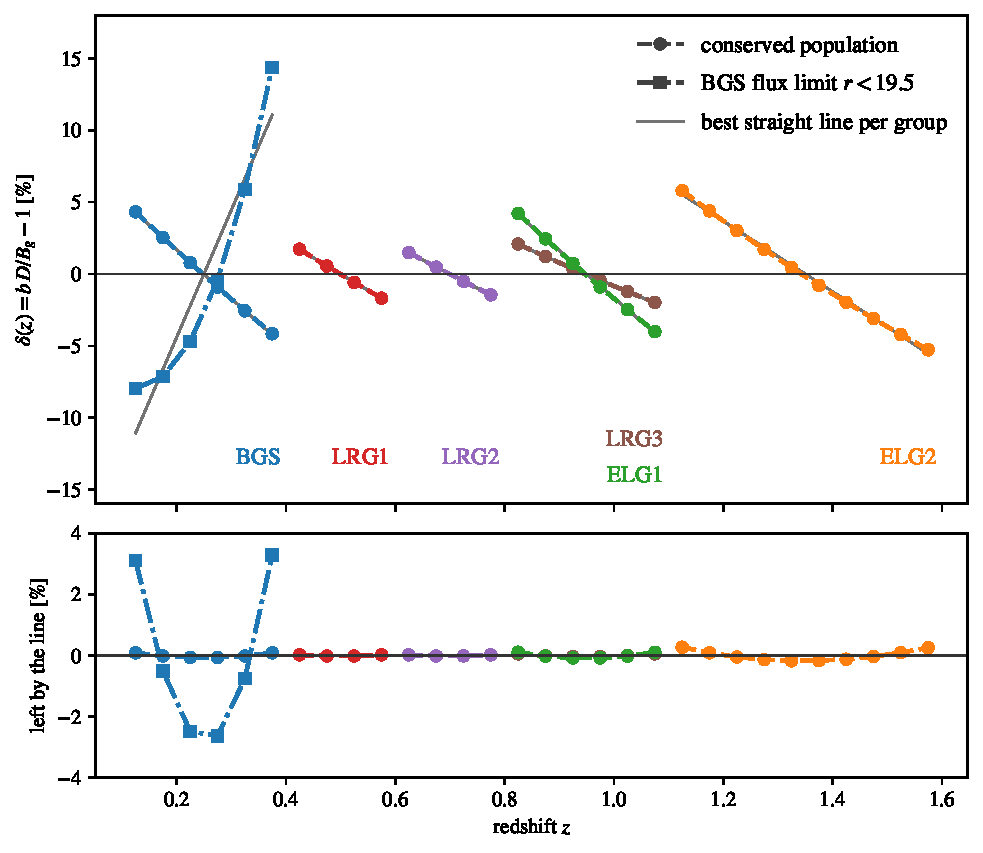
\includegraphics[width=\linewidth]{plots/theory_delta/theory_delta.pdf}
  \caption{Top: the deviation $\delta(z) = b\,D/B_g - 1$ at the
    $\Delta z = 0.05$ bin centers, with $B_g$ set so the mean deviation
    vanishes.  Dashed with circles: the conserved population, every
    group.  Dash-dot with squares: the BGS flux limit.  Thin gray: the
    best straight line per curve.  Bottom: what the line leaves.}
  \label{fig:theorydelta}
\end{figure}

\subsection{What the prior charges}
\label{sec:memcharge}

With flat priors on the line's level and slope, the prior precision of
a group's bin amplitudes is (Appendix~\ref{app:memory})
\begin{equation}
  \Prec_{\rm mem}
  \;=\;
  \mathsf{Q} - \mathsf{Q}\,\mathsf{U}
  \bigl(\mathsf{U}\T \mathsf{Q}\, \mathsf{U}\bigr)^{-1}
  \mathsf{U}\T \mathsf{Q},
  \qquad
  \mathsf{Q} = \Cov^{-1},
  \qquad
  \mathsf{U} = [\,\ones,\ v\,],
  \label{eq:memproj}
\end{equation}
the construction of Eq.~\eqref{eq:projdef} with one more column.  Its
penalty is
\begin{equation}
  \delta\T \Prec_{\rm mem}\, \delta
  \;=\;
  \min_{c,\, s_g}\;
  \bigl(\delta - c\,\ones - s_g\, v\bigr)\T
  \mathsf{Q}
  \bigl(\delta - c\,\ones - s_g\, v\bigr) :
  \label{eq:memmin}
\end{equation}
the prior subtracts the best straight line and charges only the
residual.  A monotonic drift of any size costs nothing; bumps around
the line still cost, and still forget over $L$.  $\mathsf{Q}$ is
tridiagonal (Appendix~\ref{sec:general}), while the subtracted term has
rank two and is dense, because the fitted line listens to every bin.
$\Prec_{\rm mem}\mathsf{U} = 0$, $\Prec_{\rm mem}$ is positive
semidefinite with rank $n - 2$, and a group of one or two bins has
$\Prec_{\rm mem} = 0$.

\section{The bias continuity equation, step by step}
\label{app:continuity}

The matter overdensity is $\delta_m = (\rho_m - \bar\rho_m)/\bar\rho_m$,
with $\bar\rho_m(t)$ the mean density; the galaxy-count overdensity
$\delta_{\rm gal}$ is defined the same way.  Conservation of mass and of
galaxy number gives, in comoving coordinates and to linear order (the
convective term $\mathbf{v} \cdot \nabla \delta$ is second order),
\begin{equation}
  \frac{\partial \delta_m}{\partial t}
  \;=\;
  -\,\frac{1}{a}\,\nabla \cdot \mathbf{v}_m,
  \qquad
  \frac{\partial \delta_{\rm gal}}{\partial t}
  \;=\;
  -\,\frac{1}{a}\,\nabla \cdot \mathbf{v}_{\rm gal},
  \label{eq:continuity}
\end{equation}
with $t$ cosmic time and $\mathbf{v}_m$, $\mathbf{v}_{\rm gal}$ the
peculiar velocities.  On large scales galaxies fall in the same
potential as the matter and carry no pressure of their own, so
$\mathbf{v}_{\rm gal} = \mathbf{v}_m$ (no velocity bias; galaxies as
test particles in Tegmark and Peebles~\cite{TegmarkPeebles1998}).
Subtracting the two equations and integrating from $z_c$,
\begin{equation}
  \delta_{\rm gal}(z) - \delta_m(z)
  \;=\;
  \delta_{\rm gal}(z_c) - \delta_m(z_c) :
  \label{eq:frozen}
\end{equation}
the excess clumping keeps its initial value.  With
$\delta_{\rm gal}(z_c) = b_c\,\delta_m(z_c)$ and
$\delta_m(z) = \delta_m(z_c)\, D(z)/D(z_c)$,
\begin{equation}
  \delta_{\rm gal}(z)
  \;=\;
  \delta_m(z)
  \left[\,1 + \bigl(b_c - 1\bigr)\,\frac{D(z_c)}{D(z)}\,\right],
  \label{eq:appsub}
\end{equation}
and dividing by $\delta_m(z)$ gives Eq.~\eqref{eq:fry}; dividing by the
growth-tied bias gives Eq.~\eqref{eq:tilt}.  As $D$ grows the frozen
term is divided by an ever larger number, so $b \to 1$: gravity
debiases a conserved sample.

Tegmark and Peebles also allow stochastic bias, with $b$ the ratio of
the galaxy to the matter fluctuation amplitude and $\rho_{gm}$ the
correlation coefficient of the two fields.  The same argument evolves
both: with $D$ normalized to one today and the subscript zero marking
today,
\begin{equation}
  b_0 =
  \left[(1 - D)^2 + 2 D (1 - D)\, b\, \rho_{gm}
  + D^2 b^2\right]^{1/2},
  \qquad
  \rho_{gm,0} = \frac{(1 - D) + D\, b\, \rho_{gm}}{b_0},
  \label{eq:tpevol}
\end{equation}
with $b$ and $\rho_{gm}$ the values at the epoch of growth factor $D$.
Both approach one as clustering grows, and for $\rho_{gm} = 1$
Eq.~\eqref{eq:tpevol} collapses to $b_0 - 1 = (b - 1)\,D$,
Eq.~\eqref{eq:fry} again.  For a DESI sample the assumption that
breaks is conservation (Appendix~\ref{sec:selection}); no velocity
bias and linear theory hold well on the scales kept.  The script of
Appendix~\ref{app:verify} integrates Eq.~\eqref{eq:continuity} and
recovers Eq.~\eqref{eq:fry} to $2 \times 10^{-9}$.

\section{The BGS flux-limit bias model, step by step}
\label{app:bgsflux}

This appendix derives the BGS drift of the baseline prior: a $22.3\%$
span, a convex shape, and a $2.4\%$ rms residual around the best line
(the function \texttt{bgs\_flux\_limit\_bias} of
\texttt{plots/make\_theory\_data.py}).

\subsection{The four steps}
\label{sec:bgssteps}

\paragraph{Step 1: the flux limit becomes a luminosity threshold.}
BGS Bright keeps every galaxy brighter than $r = 19.5$~\cite{Hahn2023}
($r$ the magnitude band).  The apparent magnitude $r$ and the absolute
magnitude $M$ are related by
$r = M + 25 + 5\log_{10}[d_L/(h^{-1}\,{\rm Mpc})] + K(z)$, with $d_L$
the luminosity distance and $K(z)$ the K-correction, the magnitude
correction for the part of the redshifted spectrum that falls outside
the observed band~\cite{BlantonRoweis2007}.  With $K = 0$ the faintest
absolute magnitude that passes at redshift $z$ is
\begin{equation}
  M_{\rm lim}(z) - 5\log_{10} h
  \;=\;
  19.5 - 25 - 5\log_{10} \frac{d_L(z)}{h^{-1}\,{\rm Mpc}},
  \qquad
  d_L(z) \;=\; (1+z)\,\chi(z),
  \label{eq:bgsmlim}
\end{equation}
with $\chi(z)$ the comoving distance of flat $\Lambda$CDM with
$\Omega_m = 0.3$ and $h$ the Hubble constant in units of
$100$~km/s/Mpc.

\paragraph{Steps 2 and 3: each bin is a threshold sample, and the
threshold sets the bias.}
At redshift $z$ the sample holds every galaxy with
$M < M_{\rm lim}(z)$, a threshold that brightens with distance.  The
SDSS luminosity-threshold samples at $z < 0.25$~\cite{Zehavi2011}
give
\begin{equation}
  b(>L_{\rm th})
  \;=\;
  1.06 + 0.21\,(L_{\rm th}/L_*)^{1.12},
  \qquad
  L_{\rm th}/L_* \;=\; 10^{-0.4\,(M_{\rm lim} - M_*)},
  \label{eq:bgszehavi}
\end{equation}
with $M_* - 5\log_{10} h = -20.44$ the characteristic magnitude of the
SDSS $r$-band luminosity function~\cite{Blanton2003}.  The model
applies the fit at every redshift, without evolution, and reads the
published $b\,(\sigma_8/0.8)$ as $b$.

\paragraph{Step 4: the deviation from the growth-tied shape.}
Because $B_g$ is free, only the shape of $b(z)$ matters; the amplitude
makes the mean deviation over the group's bin centers vanish:
\begin{equation}
  \delta(\bar{z}_i)
  \;=\;
  \frac{b(\bar{z}_i)\,D(\bar{z}_i)}{B} - 1,
  \qquad
  B \;=\; \frac{1}{n}\sum_{j=1}^{n} b(\bar{z}_j)\,D(\bar{z}_j).
  \label{eq:bgsdelta}
\end{equation}
At the six $\Delta z = 0.05$ bin centers of BGS, $z = 0.125$ to
$0.375$, the threshold brightens from $-18.56$ to $-21.24$, so
$L_{\rm th}/L_*$ grows from $0.18$ to $2.10$ and the bias from $1.09$
to $1.54$, while $D$ falls from $0.937$ to $0.824$.  The deviation runs
from $-8.0\%$ to $+14.4\%$, the $22.3\%$ span of
Figure~\ref{fig:theorydelta}.

\subsection{Why the drift is convex}
\label{sec:bgsconvex}

The bias rises by $41\%$ while $D$ falls by $12\%$, so the deviation
inherits the shape of the bias curve, which is flat at low redshift
and steep at high redshift: below $L_*$ the term
$0.21\,(L_{\rm th}/L_*)^{1.12}$ is small against $1.06$ ($0.03$ at the
first center), the threshold crosses $L_*$ near $z = 0.27$, and beyond
it the term rises exponentially ($0.48$ at the last center).  A
straight line through a convex curve leaves a U-shaped residual,
$(+3.1, -0.5, -2.5, -2.6, -0.8, +3.3)\%$ here.  Adding a quadratic term
cuts the residual from $2.4\%$ to $0.1\%$ rms, so the $2.4\%$ is the
curvature of the drift, the one part a free tilt cannot absorb.

\subsection{What the model leaves out}
\label{sec:bgsomissions}

None of the omissions changes the qualitative shape, a smooth,
monotonic, convex rise toward the far edge of the group.
\begin{itemize}
  \item \textbf{Evolution of the threshold-bias relation.}  The bias at
    fixed luminosity grows with redshift (Eq.~\eqref{eq:fry}), which
    steepens the drift; $M_*$ brightens by $1$--$2$ magnitudes per unit
    redshift~\cite{Blanton2003}, which flattens it, but only by
    $0.3$--$0.6$ magnitudes at the last center against the $2.68$ of
    the threshold.
  \item \textbf{No K-correction.}  A positive $K$, $0.37$ magnitudes at
    $z = 0.4$ for a spectrum flat in wavelength and more for a red
    one~\cite{BlantonRoweis2007}, makes the true threshold brighter at
    high redshift and steepens the drift.
  \item \textbf{Only $r < 19.5$.}  BGS Faint, at
    $19.5 < r < 20.175$~\cite{Hahn2023}, lowers the threshold by $0.675$
    magnitudes and flattens the drift; the fiber-magnitude cut and the
    color selection change the galaxy mix in a way
    Eq.~\eqref{eq:bgszehavi} cannot follow.
\end{itemize}
The model is an order-of-magnitude estimate, not a prediction of the
measured DESI BGS bias.  Its reliable content is the shape of the drift
and its size to a factor of order unity, which is what the baseline
prior uses: $\sigma_g = 3\%$ for BGS, from the $2$--$3\%$ curvature.
 right after \appendix.  No preamble: the
% macros \ones, \Prec, \Cov and \T come from the main file.  The labels
% are shared with the mathematics appendices (appendix_math.tex).

\section{The models}
\label{sec:models}

This appendix first builds the prior without the tilt of
Eq.~\eqref{eq:summodel}: the kernel model, in which the exponential
kernel describes the whole deviation $\delta_i$ of a bin from its
group's trend.  Appendix~\ref{sec:memory} adds the free tilt, and the
kernel then describes the residual $\varepsilon_i$ around each group's
line.  In the appendices $b_i$ is the linear bias $b_{1,i}$ of bin $i$.

\subsection{Growth-tied, free, and correlated biases}
\label{sec:defs}

The growth-tied model sets $b_i = B_g/D(\bar{z}_i)$, with one free
amplitude $B_g$ per group.  The kernel model multiplies it by a
fractional deviation $\delta_i$,
\begin{align}
  b_i &\;=\; \frac{B_g}{D(\bar{z}_i)}\,\bigl(1 + \delta_i\bigr),
  \label{eq:model}
  \\
  \bigl\langle \delta_i\,\delta_j \bigr\rangle
  &\;=\; \sigma_g^2\,
  \exp\!\left(-\,\frac{|\bar{z}_i - \bar{z}_j|}{L}\right),
  \label{eq:priorkernel}
\end{align}
with $B_g$ still free (flat prior) and the prior zero across groups.
In the Fisher matrix the convenient parameters are the per-bin
amplitudes
\begin{equation}
  \beta_i \;\equiv\; B_g\,\bigl(1 + \delta_i\bigr),
  \qquad \text{fiducial } \beta_i = B_g,
  \label{eq:beta}
\end{equation}
so that $b_i = \beta_i / D(\bar{z}_i)$.  Since
$\beta_i - B_g = B_g\,\delta_i$, the prior covariance of the $\beta_i$
within one group is
\begin{equation}
  \Cov \;=\; \sigma_\beta^2\,\mathsf{R},
  \qquad
  \sigma_\beta \;=\; \sigma_g\,B_g,
  \qquad
  \mathsf{R}_{ij} \;=\; \exp\!\left(-\,\frac{|\bar{z}_i - \bar{z}_j|}{L}\right),
  \label{eq:covdef}
\end{equation}
with $\sigma_\beta$ the spread of one amplitude, in units of a bias, and
$\mathsf{R}$ the dimensionless correlation matrix.

\subsection{What $\sigma_g$ and $L$ mean}
\label{sec:jump}

The diagonal of the kernel gives the wander of a single bin,
$\mathrm{Var}(\delta_i) = \sigma_g^2$.  The correlation coefficient of
two bins at separation $\Delta z = |\bar{z}_i - \bar{z}_j|$ is
\begin{equation}
  r \;=\;
  \frac{\langle \delta_i \delta_j \rangle}
       {\sqrt{\langle \delta_i^2 \rangle\,\langle \delta_j^2 \rangle}}
  \;=\; e^{-\Delta z / L} ,
  \label{eq:rdef}
\end{equation}
set by the separation and $L$ alone.  The jump between the two bins has
variance
\begin{equation}
  \mathrm{Var}(\delta_i - \delta_j)
  \;=\;
  2\,\sigma_g^2\left(1 - e^{-\Delta z / L}\right)
  \;\approx\;
  \frac{2\,\sigma_g^2\,\Delta z}{L}
  \quad (\Delta z \ll L).
  \label{eq:jumpvar}
\end{equation}
At small separations the jump variance grows linearly with
$\Delta z$, as for a random walk; only beyond $L$ does the finite
wander pull the deviation back.  For neighbors at $\Delta z = 0.02$
with $L = 0.05$, $r = e^{-0.4} = 0.670$ and the exact rms jump is
$0.81\,\sigma_g$; the small-separation form gives $0.89\,\sigma_g$,
because $\Delta z/L = 0.4$ is not small.

\subsection{The free group amplitude and the projection}
\label{sec:projintro}

A plain Gaussian prior with covariance $\Cov$ would charge for moving
all $\beta_i$ of a group together, but that uniform shift is the free
amplitude $B_g$.  The repair removes the uniform direction: with
$\ones$ the ones vector of the group's $n$ bins, the prior precision
of a group's amplitudes is
\begin{equation}
  \Prec \;=\; \Cov^{-1}
  \;-\;
  \frac{\Cov^{-1}\ones\,\ones\T \Cov^{-1}}{\ones\T \Cov^{-1} \ones}.
  \label{eq:projdef}
\end{equation}
$\Prec\,\ones = 0$, so a uniform shift costs nothing; a pure shape
change keeps the penalty of the plain prior; $\Prec$ is positive
semidefinite (no displacement has a negative penalty) with rank
$n - 1$; and $\Prec$ is exactly the prior
obtained by sampling $B_g$ with a flat prior and marginalizing it.
Appendices~\ref{sec:twobins}, \ref{sec:threeviews} and
\ref{sec:general} show these for two bins, by marginalization, and for
$n$ bins.  Across groups the prior is zero, so the full prior
precision is block diagonal.

\section{Which $L$ and $\sigma_g$ are physical}
\label{sec:physical}

One case of bias evolution can be solved in closed form: a population
whose members are conserved.  This appendix derives it, measures its
deviation from the growth-tied trend, lists what breaks conservation in
a selected sample, and weighs the published measurements.

\subsection{A conserved population: the bias continuity equation}
\label{sec:conserved}

Take a sample whose membership never changes, with no velocity bias,
in linear theory.  The matter overdensity $\delta_m$ and the
galaxy-count overdensity $\delta_{\rm gal}$ then obey the same
continuity equation with the same velocity field, so the excess
clumping $\delta_{\rm gal} - \delta_m$ is frozen
(Appendix~\ref{app:continuity}).  With $b_c$ the linear bias at a
reference redshift $z_c$ and $\delta_m \propto D$, the frozen
difference gives~\cite{Fry1996}
\begin{equation}
  b(z) - 1
  \;=\;
  \bigl(b_c - 1\bigr)\,\frac{D(z_c)}{D(z)} :
  \label{eq:fry}
\end{equation}
the excess set at formation stays fixed while the matter clustering
grows, so the bias decays toward one.  The growth-tied shape freezes a
different quantity: constant $b\,D$ means a galaxy clustering amplitude
$b\,\delta_m$ that does not grow, which describes a selection that
picks, at each redshift, a different and rarer set of objects.

\subsection{The deviation from the growth-tied trend}
\label{sec:tilt}

Place the reference at a group's midpoint $z_c$, with
$b_c = B/D(z_c)$.  The ratio of Eq.~\eqref{eq:fry} to the growth-tied
bias $b_c\,D(z_c)/D(z)$ gives the deviation of Eq.~\eqref{eq:model},
\begin{equation}
  \delta(z)
  \;=\;
  \frac{D(z)/D(z_c) - 1}{b_c} ,
  \label{eq:tilt}
\end{equation}
zero at the midpoint, positive at lower redshift and negative at higher
redshift, and nearly linear across a group because $D$ is smooth.  In
flat $\Lambda$CDM with $\Omega_m = 0.3$ and the project's fiducial
amplitudes it is $+5.3\%$ and $-4.9\%$ at the ends of BGS ($B = 1.34$,
$0.1 < z < 0.4$, $b_c = 1.5$), $+2.4\%$ and $-2.2\%$ at the ends of LRG1
($B = 1.70$, $0.4 < z < 0.6$, $b_c = 2.2$), and $+2.6\%$ and $-2.3\%$ at
the ends of LRG3 ($B = 1.70$, $0.8 < z < 1.1$, $b_c = 2.7$).  Between
neighbors it changes by $0.3$--$0.7\%$ at $\Delta z = 0.02$ and
$0.8$--$1.7\%$ at $\Delta z = 0.05$: a smooth tilt, coherent over the
whole group.  For comparison, the neighbor rms of
Eq.~\eqref{eq:jumpvar} at $\Delta z = 0.02$ (and $0.05$) is $2.4\%$
($3.4\%$) for $\sigma_g = 3\%$ and $L = 0.05$, and $0.44\%$ ($0.67\%$)
for $\sigma_g = 1\%$ and $L = 0.2$.  Figure~\ref{fig:theorybz} draws
these shapes: the conserved curve is flatter than $B_g/D$ in every
group, while the BGS flux-limit curve is much steeper, and convex.

\begin{figure}[htbp]
  \centering
  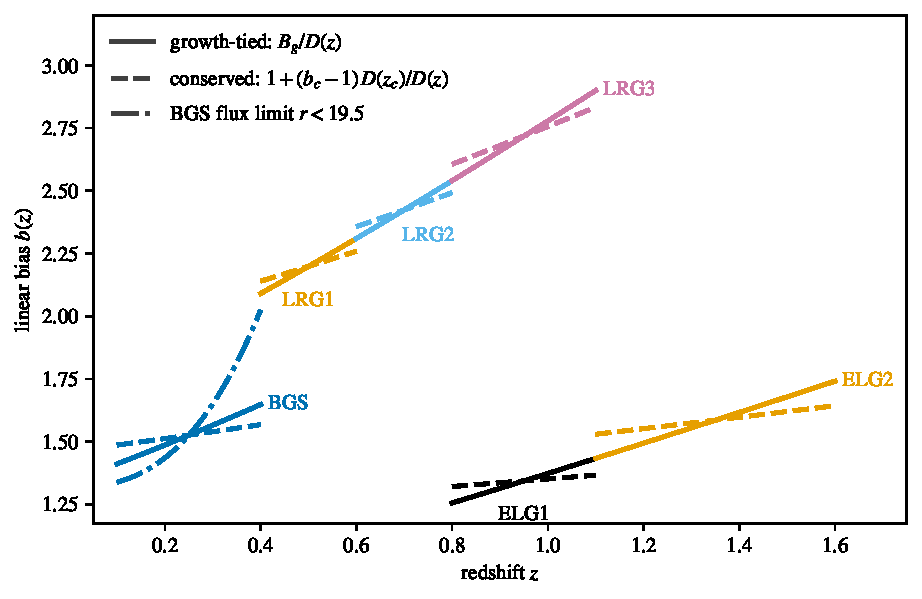
\includegraphics[width=\linewidth]{plots/theory_bz/theory_bz.pdf}
  \caption{The bias $b(z)$ of every group.  Solid: the growth-tied
    shape $B_g/D(z)$.  Dashed: a conserved population anchored at the
    group midpoint (Eq.~\eqref{eq:fry}).  Dash-dot, on BGS only: the
    $r < 19.5$ flux-limit bias, anchored at the same midpoint.}
  \label{fig:theorybz}
\end{figure}

\subsection{What breaks conservation in a selected sample}
\label{sec:selection}

\begin{itemize}
  \item \textbf{Threshold drift.}  A selection holds a roughly constant
    comoving density until the flux limit bites; beyond, it keeps only
    its brighter, more biased members.  The change is smooth, with $L$
    comparable to the group width.
  \item \textbf{Color-selection features.}  A spectral feature crossing
    a filter edge moves a color cut quickly in redshift.  The sharpest
    is the $4000$~\AA\ break, the step in an old galaxy's rest-frame
    spectrum at $4000$~\AA, which redshift slides across the filters: a
    filter edge $100$--$200$~\AA\ wide maps to
    $\Delta z = \Delta\lambda/(4000~\text{\AA}) \approx 0.03$--$0.05$.  The crossing is known; its
    amplitude in bias is unmeasured.
  \item \textbf{Mergers} turn two members into one.
  \item \textbf{Emission-line selection.}  An ELG belongs to the sample
    while its lines are strong, so membership follows the
    star-formation phase.
\end{itemize}

\subsection{What the measurements say}
\label{sec:evidence}

Each statement is tagged \emph{measured} (read from the cited source),
\emph{derived} (computed here from measured inputs) or \emph{assumed}.
Equation~\eqref{eq:fry} is from Fry~\cite{Fry1996};
Tegmark and Peebles~\cite{TegmarkPeebles1998} rederive it.

\paragraph{Massive red galaxies follow the conserved shape.}
SDSS and 2SLAQ LRGs at $0.19 < z < 0.55$, matched in color and
luminosity, show no significant evolution of the clustering amplitude
and merge at $7.5 \pm 2.3\%$ over that range, about $2.4\%$ per
Gyr~\cite{Wake2008} (measured).  The BOSS progenitors of the SDSS LRGs
merge at $2 \pm 1.5\%$ per Gyr and cluster as the continuity equation
predicts~\cite{Tojeiro2012}, and CMASS samples of fixed comoving
density at $0.43 < z < 0.7$ cluster like a conserved
population~\cite{Guo2013} (measured).  The bias of DESI-like LRGs in
photometric bins of $\Delta z \approx 0.1$ stays within $\pm 2.3\%$ of
$b = 1.5/D$ below $z = 0.83$, with the highest bin $6.4 \pm 6.4\%$
high~\cite{Zhou2021} (measured biases, residuals derived;
Figure~\ref{fig:zhou}).

\begin{figure}[htbp]
  \centering
  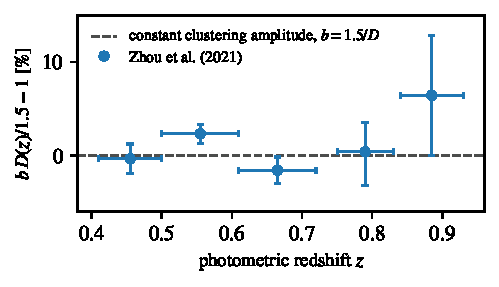
\includegraphics{plots/zhou_lrg_bias/zhou_lrg_bias.pdf}
  \caption{The measured bias of DESI-like LRGs~\cite{Zhou2021} as a
    fractional residual around $b = 1.5/D$, with $D$ at each
    photometric bin's center (flat $\Lambda$CDM, $\Omega_m = 0.3$);
    horizontal bars: the bin edges.}
  \label{fig:zhou}
\end{figure}

\paragraph{The selections drift.}
The DESI LRG cuts hold the comoving density near
$5 \times 10^{-4}\,(h/{\rm Mpc})^3$ at $0.4 < z < 0.8$ and hand over to
a fixed flux limit beyond~\cite{Zhou2023lrg} (measured).  That limit
raises the luminosity threshold by $0.27$ magnitudes per
$\Delta z = 0.1$ at $z \approx 1$; times the threshold-bias slope of
SDSS luminosity-threshold samples, $b\,(\sigma_8/0.8) = 1.06 +
0.21\,(L_{\rm th}/L_*)^{1.12}$~\cite{Zehavi2011} ($0.5$--$1.0$ in bias
per magnitude near LRG luminosities; measured), it drifts the LRG3 bias
by $6$--$11\%$ per $\Delta z = 0.1$ on top of $B/D$ (derived, from an
$r$-band relation outside its calibrated range, so only the direction
and order of magnitude hold).  BGS Bright is magnitude limited at
$r < 19.5$~\cite{Hahn2023} (measured), which drives a $10$--$25\%$ bias
drift across the group (derived; Appendix~\ref{app:bgsflux}).

\paragraph{The ELG bias shape is stable.}
Fits of the halo occupation distribution (HOD: how many sample
galaxies live in a halo of each mass) to the DESI One-Percent ELGs in
$0.8 < z < 1.1$ and
$1.1 < z < 1.6$ agree within one sigma~\cite{Rocher2023} (measured);
at these host masses the halo bias depends weakly on mass, so the
implied drift is at the percent level (derived, slope assumed).  The
[OII] doublet loses signal-to-noise in windows
$\Delta z \approx 0.001$--$0.01$ wide where it lands on sky lines,
especially at $z > 1.5$~\cite{Raichoor2023} (measured): the one
short-separation mechanism with a measured location, with an assumed
bias amplitude of $1$--$2\%$.

\paragraph{Nothing resolves bias below $\Delta z \approx 0.1$.}
The CMB-lensing tomography of the same samples~\cite{White2022,
Sailer2024, Sailer2025}, on the photometric samples of
Zhou et al.~\cite{Zhou2023tomo}, uses bins of about $0.15$ with one
free bias per bin and finds smooth models that fit.  Below
$\Delta z \approx 0.1$ this note rests on the continuity equation and
the selection arguments.

\section{The memory model}
\label{sec:memory}

\subsection{Why a second model}
\label{sec:memwhy}

Every deviation above except the sky-line windows is a monotonic drift:
the conserved-population tilt (about $1\%$ per $\Delta z = 0.05$), the
LRG3 magnitude-limit drift ($6$--$11\%$ per $\Delta z = 0.1$) and the
BGS flux-limit drift ($10$--$25\%$ across the group).  The kernel model
admits such a drift only at a price: to pass a $20\%$ drift with
$L \leq 0.1$ it takes $\sigma_g = 10$--$15\%$, which also allows about
$10\%$ scatter between neighbors that no identified mechanism
produces.  One $\sigma_g$ controls both, so the kernel cannot say
``large smooth drift, small local scatter''.  The memory model
separates the two.

\subsection{Why the kernel forgets}
\label{sec:memforget}

At $L = 0.05$, bins $0.15$ apart share $e^{-3} \approx 0.05$ of their
deviation.  With $r_k = e^{-(\bar{z}_{k+1} - \bar{z}_k)/L}$ the
correlation of neighbors $k$ and $k+1$, the best guess of the next bin
given all earlier ones is (Appendix~\ref{app:chain})
\begin{equation}
  \mathrm{E}\bigl[\delta_{k+1} \mid \delta_1, \dots, \delta_k\bigr]
  \;=\; r_k\, \delta_k :
  \label{eq:memmarkov}
\end{equation}
only the nearest neighbor matters, and the influence of any one bin
fades along the chain.

\subsection{The model, and why it remembers}
\label{sec:memmodel}

The memory model adds a tilt per group and splits the deviation into a
line and a residual,
\begin{equation}
  \delta_i \;=\; s_g\, v_i + \varepsilon_i,
  \qquad
  v_i \;=\; \bar{z}_i - \bar{z}_g,
  \label{eq:memdef}
\end{equation}
with $s_g$ a free tilt (flat prior, like $B_g$) and $\varepsilon_i$
carrying the kernel of Eq.~\eqref{eq:priorkernel}: the model of
Eqs.~\eqref{eq:summodel} and \eqref{eq:sumkernel}.  Giving the slope a
Gaussian prior of variance $\tau^2$ first (the flat prior is
$\tau \to \infty$), the deviations have covariance
\begin{equation}
  \mathrm{Cov}(\delta_i, \delta_j)
  \;=\;
  \tau^2\, v_i\, v_j
  \;+\;
  \sigma_g^2\, e^{-|\bar{z}_i - \bar{z}_j|/L} .
  \label{eq:memcov}
\end{equation}
The new term does not decay with separation.  Far beyond $L$ the
correlation coefficient tends to
\begin{equation}
  \rho_{ij}
  \;\longrightarrow\;
  \frac{\tau^2 v_i v_j}
       {\sqrt{\bigl(\tau^2 v_i^2 + \sigma_g^2\bigr)
              \bigl(\tau^2 v_j^2 + \sigma_g^2\bigr)}}
  \;\longrightarrow\; \pm 1
  \quad \text{when } \tau |v| \gg \sigma_g :
  \label{eq:memrho}
\end{equation}
the two ends of a group remember each other through the shared slope.
The best guess of the next bin becomes
\begin{equation}
  \mathrm{E}\bigl[\delta_{k+1} \mid \delta_1, \dots, \delta_k\bigr]
  \;=\;
  \hat{c} + \hat{s}_g\, v_{k+1}
  \;+\;
  r_k\,\bigl(\delta_k - \hat{c} - \hat{s}_g\, v_k\bigr),
  \label{eq:memkriging}
\end{equation}
with $(\hat{c}, \hat{s}_g)$ the level and slope of the best straight
line through all past bins, weighted by $\Cov^{-1}$: every past bin
enters through the fitted line, and only the wiggle around it stays
Markov (the universal-kriging predictor; kriging is the geostatistics
name for the best linear prediction from correlated data;
Appendix~\ref{app:memory}).
Figure~\ref{fig:theorydraws} shows the difference on the BGS bins at
$\Delta z = 0.02$: kernel draws wide enough to admit the BGS drift
zigzag and forget, while memory draws are lines with small wiggles,
among which the drift looks typical.

\begin{figure}[htbp]
  \centering
  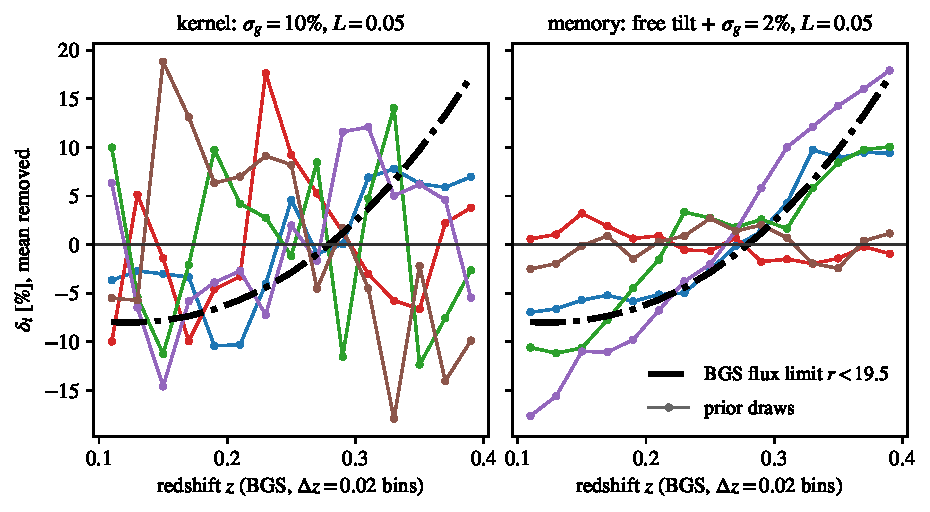
\includegraphics[width=\linewidth]{plots/theory_draws/theory_draws.pdf}
  \caption{Random prior draws of the deviations of the 15 BGS bins at
    $\Delta z = 0.02$, each draw's mean removed ($B_g$ is free).  Thick
    dash-dot: the BGS flux-limit drift.  Left: the kernel model.
    Right: the memory model, whose tilt is free in the model and drawn
    here, for display only, from a Gaussian of width $0.6$ per unit
    redshift.}
  \label{fig:theorydraws}
\end{figure}

\subsection{Why the memory model differs physically}
\label{sec:memphysics}

A selected sample changes along a group in two ways.  Coherent changes
move every bin the same way: a threshold that rises with distance, the
debiasing of a conserved population.  Local changes move bins
independently and are forgotten over a short range: the sky-line
windows and filter-edge crossings of Appendix~\ref{sec:selection}.  The
memory model gives the first kind to the tilt and the second to the
kernel.  One line suffices for the coherent kind, because the drifts
are smooth functions of $D(z)$ and the distance modulus.  The best
equal-weight line through each group's conserved deviation at the
$\Delta z = 0.05$ bin centers (derived; amplitudes $1.34$ for BGS,
$1.70$ for the LRGs and $0.84$ for the ELGs) removes deviations that
span $3$--$11\%$ and leaves $0.02$--$0.16\%$ rms, at most $0.27\%$
(ELG2).  The BGS flux-limit drift is larger and convex: it spans
$22.3\%$, and its best line leaves $2.4\%$ rms and $3.3\%$ at most
(Appendix~\ref{app:bgsflux}).  Figure~\ref{fig:theorydelta} shows both.
In the memory model $\sigma_g$ is the departure from the group's own
line, curvature plus local scatter: about $0.1\%$ for a conserved
population, $1$--$2\%$ for local selection features, $2$--$3\%$ for the
BGS curvature.

\begin{figure}[htbp]
  \centering
  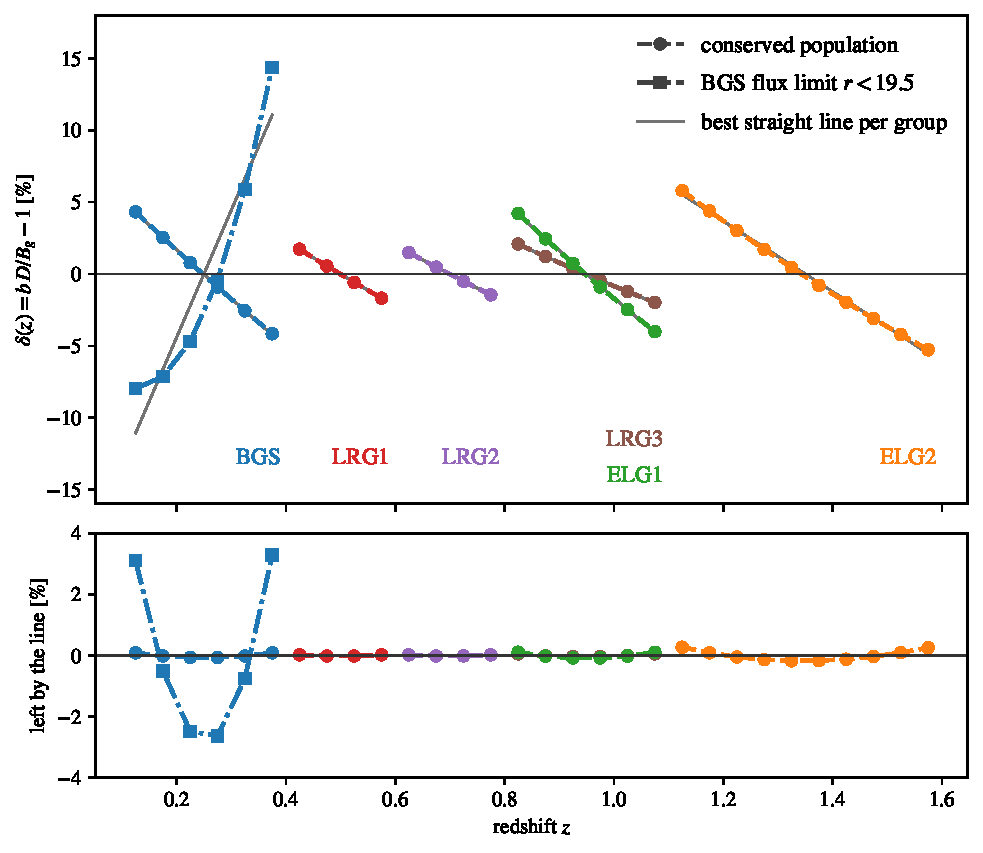
\includegraphics[width=\linewidth]{plots/theory_delta/theory_delta.pdf}
  \caption{Top: the deviation $\delta(z) = b\,D/B_g - 1$ at the
    $\Delta z = 0.05$ bin centers, with $B_g$ set so the mean deviation
    vanishes.  Dashed with circles: the conserved population, every
    group.  Dash-dot with squares: the BGS flux limit.  Thin gray: the
    best straight line per curve.  Bottom: what the line leaves.}
  \label{fig:theorydelta}
\end{figure}

\subsection{What the prior charges}
\label{sec:memcharge}

With flat priors on the line's level and slope, the prior precision of
a group's bin amplitudes is (Appendix~\ref{app:memory})
\begin{equation}
  \Prec_{\rm mem}
  \;=\;
  \mathsf{Q} - \mathsf{Q}\,\mathsf{U}
  \bigl(\mathsf{U}\T \mathsf{Q}\, \mathsf{U}\bigr)^{-1}
  \mathsf{U}\T \mathsf{Q},
  \qquad
  \mathsf{Q} = \Cov^{-1},
  \qquad
  \mathsf{U} = [\,\ones,\ v\,],
  \label{eq:memproj}
\end{equation}
the construction of Eq.~\eqref{eq:projdef} with one more column.  Its
penalty is
\begin{equation}
  \delta\T \Prec_{\rm mem}\, \delta
  \;=\;
  \min_{c,\, s_g}\;
  \bigl(\delta - c\,\ones - s_g\, v\bigr)\T
  \mathsf{Q}
  \bigl(\delta - c\,\ones - s_g\, v\bigr) :
  \label{eq:memmin}
\end{equation}
the prior subtracts the best straight line and charges only the
residual.  A monotonic drift of any size costs nothing; bumps around
the line still cost, and still forget over $L$.  $\mathsf{Q}$ is
tridiagonal (Appendix~\ref{sec:general}), while the subtracted term has
rank two and is dense, because the fitted line listens to every bin.
$\Prec_{\rm mem}\mathsf{U} = 0$, $\Prec_{\rm mem}$ is positive
semidefinite with rank $n - 2$, and a group of one or two bins has
$\Prec_{\rm mem} = 0$.

\section{The bias continuity equation, step by step}
\label{app:continuity}

The matter overdensity is $\delta_m = (\rho_m - \bar\rho_m)/\bar\rho_m$,
with $\bar\rho_m(t)$ the mean density; the galaxy-count overdensity
$\delta_{\rm gal}$ is defined the same way.  Conservation of mass and of
galaxy number gives, in comoving coordinates and to linear order (the
convective term $\mathbf{v} \cdot \nabla \delta$ is second order),
\begin{equation}
  \frac{\partial \delta_m}{\partial t}
  \;=\;
  -\,\frac{1}{a}\,\nabla \cdot \mathbf{v}_m,
  \qquad
  \frac{\partial \delta_{\rm gal}}{\partial t}
  \;=\;
  -\,\frac{1}{a}\,\nabla \cdot \mathbf{v}_{\rm gal},
  \label{eq:continuity}
\end{equation}
with $t$ cosmic time and $\mathbf{v}_m$, $\mathbf{v}_{\rm gal}$ the
peculiar velocities.  On large scales galaxies fall in the same
potential as the matter and carry no pressure of their own, so
$\mathbf{v}_{\rm gal} = \mathbf{v}_m$ (no velocity bias; galaxies as
test particles in Tegmark and Peebles~\cite{TegmarkPeebles1998}).
Subtracting the two equations and integrating from $z_c$,
\begin{equation}
  \delta_{\rm gal}(z) - \delta_m(z)
  \;=\;
  \delta_{\rm gal}(z_c) - \delta_m(z_c) :
  \label{eq:frozen}
\end{equation}
the excess clumping keeps its initial value.  With
$\delta_{\rm gal}(z_c) = b_c\,\delta_m(z_c)$ and
$\delta_m(z) = \delta_m(z_c)\, D(z)/D(z_c)$,
\begin{equation}
  \delta_{\rm gal}(z)
  \;=\;
  \delta_m(z)
  \left[\,1 + \bigl(b_c - 1\bigr)\,\frac{D(z_c)}{D(z)}\,\right],
  \label{eq:appsub}
\end{equation}
and dividing by $\delta_m(z)$ gives Eq.~\eqref{eq:fry}; dividing by the
growth-tied bias gives Eq.~\eqref{eq:tilt}.  As $D$ grows the frozen
term is divided by an ever larger number, so $b \to 1$: gravity
debiases a conserved sample.

Tegmark and Peebles also allow stochastic bias, with $b$ the ratio of
the galaxy to the matter fluctuation amplitude and $\rho_{gm}$ the
correlation coefficient of the two fields.  The same argument evolves
both: with $D$ normalized to one today and the subscript zero marking
today,
\begin{equation}
  b_0 =
  \left[(1 - D)^2 + 2 D (1 - D)\, b\, \rho_{gm}
  + D^2 b^2\right]^{1/2},
  \qquad
  \rho_{gm,0} = \frac{(1 - D) + D\, b\, \rho_{gm}}{b_0},
  \label{eq:tpevol}
\end{equation}
with $b$ and $\rho_{gm}$ the values at the epoch of growth factor $D$.
Both approach one as clustering grows, and for $\rho_{gm} = 1$
Eq.~\eqref{eq:tpevol} collapses to $b_0 - 1 = (b - 1)\,D$,
Eq.~\eqref{eq:fry} again.  For a DESI sample the assumption that
breaks is conservation (Appendix~\ref{sec:selection}); no velocity
bias and linear theory hold well on the scales kept.  The script of
Appendix~\ref{app:verify} integrates Eq.~\eqref{eq:continuity} and
recovers Eq.~\eqref{eq:fry} to $2 \times 10^{-9}$.

\section{The BGS flux-limit bias model, step by step}
\label{app:bgsflux}

This appendix derives the BGS drift of the baseline prior: a $22.3\%$
span, a convex shape, and a $2.4\%$ rms residual around the best line
(the function \texttt{bgs\_flux\_limit\_bias} of
\texttt{plots/make\_theory\_data.py}).

\subsection{The four steps}
\label{sec:bgssteps}

\paragraph{Step 1: the flux limit becomes a luminosity threshold.}
BGS Bright keeps every galaxy brighter than $r = 19.5$~\cite{Hahn2023}
($r$ the magnitude band).  The apparent magnitude $r$ and the absolute
magnitude $M$ are related by
$r = M + 25 + 5\log_{10}[d_L/(h^{-1}\,{\rm Mpc})] + K(z)$, with $d_L$
the luminosity distance and $K(z)$ the K-correction, the magnitude
correction for the part of the redshifted spectrum that falls outside
the observed band~\cite{BlantonRoweis2007}.  With $K = 0$ the faintest
absolute magnitude that passes at redshift $z$ is
\begin{equation}
  M_{\rm lim}(z) - 5\log_{10} h
  \;=\;
  19.5 - 25 - 5\log_{10} \frac{d_L(z)}{h^{-1}\,{\rm Mpc}},
  \qquad
  d_L(z) \;=\; (1+z)\,\chi(z),
  \label{eq:bgsmlim}
\end{equation}
with $\chi(z)$ the comoving distance of flat $\Lambda$CDM with
$\Omega_m = 0.3$ and $h$ the Hubble constant in units of
$100$~km/s/Mpc.

\paragraph{Steps 2 and 3: each bin is a threshold sample, and the
threshold sets the bias.}
At redshift $z$ the sample holds every galaxy with
$M < M_{\rm lim}(z)$, a threshold that brightens with distance.  The
SDSS luminosity-threshold samples at $z < 0.25$~\cite{Zehavi2011}
give
\begin{equation}
  b(>L_{\rm th})
  \;=\;
  1.06 + 0.21\,(L_{\rm th}/L_*)^{1.12},
  \qquad
  L_{\rm th}/L_* \;=\; 10^{-0.4\,(M_{\rm lim} - M_*)},
  \label{eq:bgszehavi}
\end{equation}
with $M_* - 5\log_{10} h = -20.44$ the characteristic magnitude of the
SDSS $r$-band luminosity function~\cite{Blanton2003}.  The model
applies the fit at every redshift, without evolution, and reads the
published $b\,(\sigma_8/0.8)$ as $b$.

\paragraph{Step 4: the deviation from the growth-tied shape.}
Because $B_g$ is free, only the shape of $b(z)$ matters; the amplitude
makes the mean deviation over the group's bin centers vanish:
\begin{equation}
  \delta(\bar{z}_i)
  \;=\;
  \frac{b(\bar{z}_i)\,D(\bar{z}_i)}{B} - 1,
  \qquad
  B \;=\; \frac{1}{n}\sum_{j=1}^{n} b(\bar{z}_j)\,D(\bar{z}_j).
  \label{eq:bgsdelta}
\end{equation}
At the six $\Delta z = 0.05$ bin centers of BGS, $z = 0.125$ to
$0.375$, the threshold brightens from $-18.56$ to $-21.24$, so
$L_{\rm th}/L_*$ grows from $0.18$ to $2.10$ and the bias from $1.09$
to $1.54$, while $D$ falls from $0.937$ to $0.824$.  The deviation runs
from $-8.0\%$ to $+14.4\%$, the $22.3\%$ span of
Figure~\ref{fig:theorydelta}.

\subsection{Why the drift is convex}
\label{sec:bgsconvex}

The bias rises by $41\%$ while $D$ falls by $12\%$, so the deviation
inherits the shape of the bias curve, which is flat at low redshift
and steep at high redshift: below $L_*$ the term
$0.21\,(L_{\rm th}/L_*)^{1.12}$ is small against $1.06$ ($0.03$ at the
first center), the threshold crosses $L_*$ near $z = 0.27$, and beyond
it the term rises exponentially ($0.48$ at the last center).  A
straight line through a convex curve leaves a U-shaped residual,
$(+3.1, -0.5, -2.5, -2.6, -0.8, +3.3)\%$ here.  Adding a quadratic term
cuts the residual from $2.4\%$ to $0.1\%$ rms, so the $2.4\%$ is the
curvature of the drift, the one part a free tilt cannot absorb.

\subsection{What the model leaves out}
\label{sec:bgsomissions}

None of the omissions changes the qualitative shape, a smooth,
monotonic, convex rise toward the far edge of the group.
\begin{itemize}
  \item \textbf{Evolution of the threshold-bias relation.}  The bias at
    fixed luminosity grows with redshift (Eq.~\eqref{eq:fry}), which
    steepens the drift; $M_*$ brightens by $1$--$2$ magnitudes per unit
    redshift~\cite{Blanton2003}, which flattens it, but only by
    $0.3$--$0.6$ magnitudes at the last center against the $2.68$ of
    the threshold.
  \item \textbf{No K-correction.}  A positive $K$, $0.37$ magnitudes at
    $z = 0.4$ for a spectrum flat in wavelength and more for a red
    one~\cite{BlantonRoweis2007}, makes the true threshold brighter at
    high redshift and steepens the drift.
  \item \textbf{Only $r < 19.5$.}  BGS Faint, at
    $19.5 < r < 20.175$~\cite{Hahn2023}, lowers the threshold by $0.675$
    magnitudes and flattens the drift; the fiber-magnitude cut and the
    color selection change the galaxy mix in a way
    Eq.~\eqref{eq:bgszehavi} cannot follow.
\end{itemize}
The model is an order-of-magnitude estimate, not a prediction of the
measured DESI BGS bias.  Its reliable content is the shape of the drift
and its size to a factor of order unity, which is what the baseline
prior uses: $\sigma_g = 3\%$ for BGS, from the $2$--$3\%$ curvature.
 right after \appendix.  No preamble: the
% macros \ones, \Prec, \Cov and \T come from the main file.  The labels
% are shared with the mathematics appendices (appendix_math.tex).

\section{The models}
\label{sec:models}

This appendix first builds the prior without the tilt of
Eq.~\eqref{eq:summodel}: the kernel model, in which the exponential
kernel describes the whole deviation $\delta_i$ of a bin from its
group's trend.  Appendix~\ref{sec:memory} adds the free tilt, and the
kernel then describes the residual $\varepsilon_i$ around each group's
line.  In the appendices $b_i$ is the linear bias $b_{1,i}$ of bin $i$.

\subsection{Growth-tied, free, and correlated biases}
\label{sec:defs}

The growth-tied model sets $b_i = B_g/D(\bar{z}_i)$, with one free
amplitude $B_g$ per group.  The kernel model multiplies it by a
fractional deviation $\delta_i$,
\begin{align}
  b_i &\;=\; \frac{B_g}{D(\bar{z}_i)}\,\bigl(1 + \delta_i\bigr),
  \label{eq:model}
  \\
  \bigl\langle \delta_i\,\delta_j \bigr\rangle
  &\;=\; \sigma_g^2\,
  \exp\!\left(-\,\frac{|\bar{z}_i - \bar{z}_j|}{L}\right),
  \label{eq:priorkernel}
\end{align}
with $B_g$ still free (flat prior) and the prior zero across groups.
In the Fisher matrix the convenient parameters are the per-bin
amplitudes
\begin{equation}
  \beta_i \;\equiv\; B_g\,\bigl(1 + \delta_i\bigr),
  \qquad \text{fiducial } \beta_i = B_g,
  \label{eq:beta}
\end{equation}
so that $b_i = \beta_i / D(\bar{z}_i)$.  Since
$\beta_i - B_g = B_g\,\delta_i$, the prior covariance of the $\beta_i$
within one group is
\begin{equation}
  \Cov \;=\; \sigma_\beta^2\,\mathsf{R},
  \qquad
  \sigma_\beta \;=\; \sigma_g\,B_g,
  \qquad
  \mathsf{R}_{ij} \;=\; \exp\!\left(-\,\frac{|\bar{z}_i - \bar{z}_j|}{L}\right),
  \label{eq:covdef}
\end{equation}
with $\sigma_\beta$ the spread of one amplitude, in units of a bias, and
$\mathsf{R}$ the dimensionless correlation matrix.

\subsection{What $\sigma_g$ and $L$ mean}
\label{sec:jump}

The diagonal of the kernel gives the wander of a single bin,
$\mathrm{Var}(\delta_i) = \sigma_g^2$.  The correlation coefficient of
two bins at separation $\Delta z = |\bar{z}_i - \bar{z}_j|$ is
\begin{equation}
  r \;=\;
  \frac{\langle \delta_i \delta_j \rangle}
       {\sqrt{\langle \delta_i^2 \rangle\,\langle \delta_j^2 \rangle}}
  \;=\; e^{-\Delta z / L} ,
  \label{eq:rdef}
\end{equation}
set by the separation and $L$ alone.  The jump between the two bins has
variance
\begin{equation}
  \mathrm{Var}(\delta_i - \delta_j)
  \;=\;
  2\,\sigma_g^2\left(1 - e^{-\Delta z / L}\right)
  \;\approx\;
  \frac{2\,\sigma_g^2\,\Delta z}{L}
  \quad (\Delta z \ll L).
  \label{eq:jumpvar}
\end{equation}
At small separations the jump variance grows linearly with
$\Delta z$, as for a random walk; only beyond $L$ does the finite
wander pull the deviation back.  For neighbors at $\Delta z = 0.02$
with $L = 0.05$, $r = e^{-0.4} = 0.670$ and the exact rms jump is
$0.81\,\sigma_g$; the small-separation form gives $0.89\,\sigma_g$,
because $\Delta z/L = 0.4$ is not small.

\subsection{The free group amplitude and the projection}
\label{sec:projintro}

A plain Gaussian prior with covariance $\Cov$ would charge for moving
all $\beta_i$ of a group together, but that uniform shift is the free
amplitude $B_g$.  The repair removes the uniform direction: with
$\ones$ the ones vector of the group's $n$ bins, the prior precision
of a group's amplitudes is
\begin{equation}
  \Prec \;=\; \Cov^{-1}
  \;-\;
  \frac{\Cov^{-1}\ones\,\ones\T \Cov^{-1}}{\ones\T \Cov^{-1} \ones}.
  \label{eq:projdef}
\end{equation}
$\Prec\,\ones = 0$, so a uniform shift costs nothing; a pure shape
change keeps the penalty of the plain prior; $\Prec$ is positive
semidefinite (no displacement has a negative penalty) with rank
$n - 1$; and $\Prec$ is exactly the prior
obtained by sampling $B_g$ with a flat prior and marginalizing it.
Appendices~\ref{sec:twobins}, \ref{sec:threeviews} and
\ref{sec:general} show these for two bins, by marginalization, and for
$n$ bins.  Across groups the prior is zero, so the full prior
precision is block diagonal.

\section{Which $L$ and $\sigma_g$ are physical}
\label{sec:physical}

One case of bias evolution can be solved in closed form: a population
whose members are conserved.  This appendix derives it, measures its
deviation from the growth-tied trend, lists what breaks conservation in
a selected sample, and weighs the published measurements.

\subsection{A conserved population: the bias continuity equation}
\label{sec:conserved}

Take a sample whose membership never changes, with no velocity bias,
in linear theory.  The matter overdensity $\delta_m$ and the
galaxy-count overdensity $\delta_{\rm gal}$ then obey the same
continuity equation with the same velocity field, so the excess
clumping $\delta_{\rm gal} - \delta_m$ is frozen
(Appendix~\ref{app:continuity}).  With $b_c$ the linear bias at a
reference redshift $z_c$ and $\delta_m \propto D$, the frozen
difference gives~\cite{Fry1996}
\begin{equation}
  b(z) - 1
  \;=\;
  \bigl(b_c - 1\bigr)\,\frac{D(z_c)}{D(z)} :
  \label{eq:fry}
\end{equation}
the excess set at formation stays fixed while the matter clustering
grows, so the bias decays toward one.  The growth-tied shape freezes a
different quantity: constant $b\,D$ means a galaxy clustering amplitude
$b\,\delta_m$ that does not grow, which describes a selection that
picks, at each redshift, a different and rarer set of objects.

\subsection{The deviation from the growth-tied trend}
\label{sec:tilt}

Place the reference at a group's midpoint $z_c$, with
$b_c = B/D(z_c)$.  The ratio of Eq.~\eqref{eq:fry} to the growth-tied
bias $b_c\,D(z_c)/D(z)$ gives the deviation of Eq.~\eqref{eq:model},
\begin{equation}
  \delta(z)
  \;=\;
  \frac{D(z)/D(z_c) - 1}{b_c} ,
  \label{eq:tilt}
\end{equation}
zero at the midpoint, positive at lower redshift and negative at higher
redshift, and nearly linear across a group because $D$ is smooth.  In
flat $\Lambda$CDM with $\Omega_m = 0.3$ and the project's fiducial
amplitudes it is $+5.3\%$ and $-4.9\%$ at the ends of BGS ($B = 1.34$,
$0.1 < z < 0.4$, $b_c = 1.5$), $+2.4\%$ and $-2.2\%$ at the ends of LRG1
($B = 1.70$, $0.4 < z < 0.6$, $b_c = 2.2$), and $+2.6\%$ and $-2.3\%$ at
the ends of LRG3 ($B = 1.70$, $0.8 < z < 1.1$, $b_c = 2.7$).  Between
neighbors it changes by $0.3$--$0.7\%$ at $\Delta z = 0.02$ and
$0.8$--$1.7\%$ at $\Delta z = 0.05$: a smooth tilt, coherent over the
whole group.  For comparison, the neighbor rms of
Eq.~\eqref{eq:jumpvar} at $\Delta z = 0.02$ (and $0.05$) is $2.4\%$
($3.4\%$) for $\sigma_g = 3\%$ and $L = 0.05$, and $0.44\%$ ($0.67\%$)
for $\sigma_g = 1\%$ and $L = 0.2$.  Figure~\ref{fig:theorybz} draws
these shapes: the conserved curve is flatter than $B_g/D$ in every
group, while the BGS flux-limit curve is much steeper, and convex.

\begin{figure}[htbp]
  \centering
  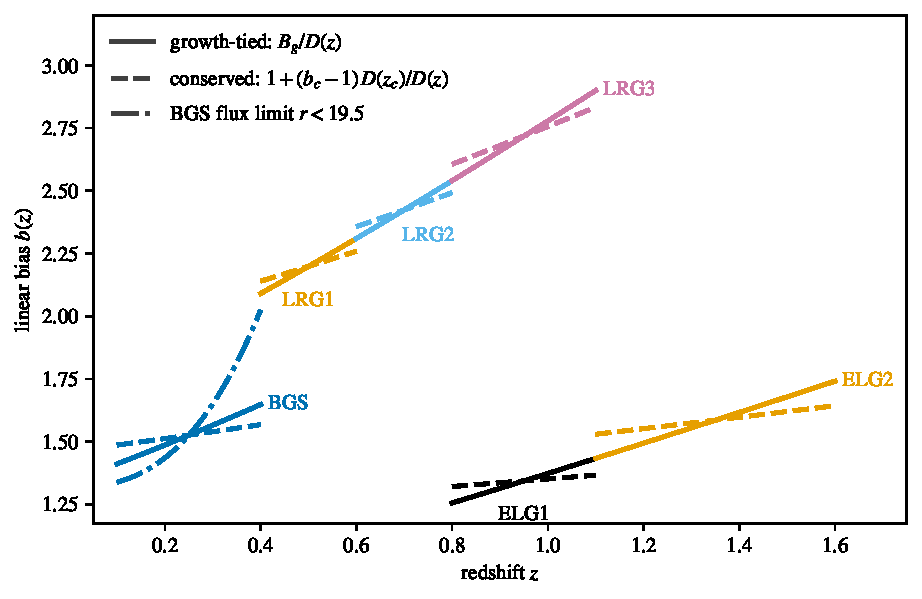
\includegraphics[width=\linewidth]{plots/theory_bz/theory_bz.pdf}
  \caption{The bias $b(z)$ of every group.  Solid: the growth-tied
    shape $B_g/D(z)$.  Dashed: a conserved population anchored at the
    group midpoint (Eq.~\eqref{eq:fry}).  Dash-dot, on BGS only: the
    $r < 19.5$ flux-limit bias, anchored at the same midpoint.}
  \label{fig:theorybz}
\end{figure}

\subsection{What breaks conservation in a selected sample}
\label{sec:selection}

\begin{itemize}
  \item \textbf{Threshold drift.}  A selection holds a roughly constant
    comoving density until the flux limit bites; beyond, it keeps only
    its brighter, more biased members.  The change is smooth, with $L$
    comparable to the group width.
  \item \textbf{Color-selection features.}  A spectral feature crossing
    a filter edge moves a color cut quickly in redshift.  The sharpest
    is the $4000$~\AA\ break, the step in an old galaxy's rest-frame
    spectrum at $4000$~\AA, which redshift slides across the filters: a
    filter edge $100$--$200$~\AA\ wide maps to
    $\Delta z = \Delta\lambda/(4000~\text{\AA}) \approx 0.03$--$0.05$.  The crossing is known; its
    amplitude in bias is unmeasured.
  \item \textbf{Mergers} turn two members into one.
  \item \textbf{Emission-line selection.}  An ELG belongs to the sample
    while its lines are strong, so membership follows the
    star-formation phase.
\end{itemize}

\subsection{What the measurements say}
\label{sec:evidence}

Each statement is tagged \emph{measured} (read from the cited source),
\emph{derived} (computed here from measured inputs) or \emph{assumed}.
Equation~\eqref{eq:fry} is from Fry~\cite{Fry1996};
Tegmark and Peebles~\cite{TegmarkPeebles1998} rederive it.

\paragraph{Massive red galaxies follow the conserved shape.}
SDSS and 2SLAQ LRGs at $0.19 < z < 0.55$, matched in color and
luminosity, show no significant evolution of the clustering amplitude
and merge at $7.5 \pm 2.3\%$ over that range, about $2.4\%$ per
Gyr~\cite{Wake2008} (measured).  The BOSS progenitors of the SDSS LRGs
merge at $2 \pm 1.5\%$ per Gyr and cluster as the continuity equation
predicts~\cite{Tojeiro2012}, and CMASS samples of fixed comoving
density at $0.43 < z < 0.7$ cluster like a conserved
population~\cite{Guo2013} (measured).  The bias of DESI-like LRGs in
photometric bins of $\Delta z \approx 0.1$ stays within $\pm 2.3\%$ of
$b = 1.5/D$ below $z = 0.83$, with the highest bin $6.4 \pm 6.4\%$
high~\cite{Zhou2021} (measured biases, residuals derived;
Figure~\ref{fig:zhou}).

\begin{figure}[htbp]
  \centering
  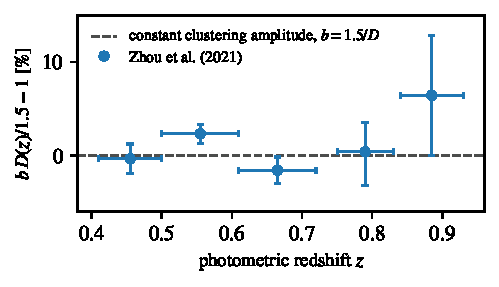
\includegraphics{plots/zhou_lrg_bias/zhou_lrg_bias.pdf}
  \caption{The measured bias of DESI-like LRGs~\cite{Zhou2021} as a
    fractional residual around $b = 1.5/D$, with $D$ at each
    photometric bin's center (flat $\Lambda$CDM, $\Omega_m = 0.3$);
    horizontal bars: the bin edges.}
  \label{fig:zhou}
\end{figure}

\paragraph{The selections drift.}
The DESI LRG cuts hold the comoving density near
$5 \times 10^{-4}\,(h/{\rm Mpc})^3$ at $0.4 < z < 0.8$ and hand over to
a fixed flux limit beyond~\cite{Zhou2023lrg} (measured).  That limit
raises the luminosity threshold by $0.27$ magnitudes per
$\Delta z = 0.1$ at $z \approx 1$; times the threshold-bias slope of
SDSS luminosity-threshold samples, $b\,(\sigma_8/0.8) = 1.06 +
0.21\,(L_{\rm th}/L_*)^{1.12}$~\cite{Zehavi2011} ($0.5$--$1.0$ in bias
per magnitude near LRG luminosities; measured), it drifts the LRG3 bias
by $6$--$11\%$ per $\Delta z = 0.1$ on top of $B/D$ (derived, from an
$r$-band relation outside its calibrated range, so only the direction
and order of magnitude hold).  BGS Bright is magnitude limited at
$r < 19.5$~\cite{Hahn2023} (measured), which drives a $10$--$25\%$ bias
drift across the group (derived; Appendix~\ref{app:bgsflux}).

\paragraph{The ELG bias shape is stable.}
Fits of the halo occupation distribution (HOD: how many sample
galaxies live in a halo of each mass) to the DESI One-Percent ELGs in
$0.8 < z < 1.1$ and
$1.1 < z < 1.6$ agree within one sigma~\cite{Rocher2023} (measured);
at these host masses the halo bias depends weakly on mass, so the
implied drift is at the percent level (derived, slope assumed).  The
[OII] doublet loses signal-to-noise in windows
$\Delta z \approx 0.001$--$0.01$ wide where it lands on sky lines,
especially at $z > 1.5$~\cite{Raichoor2023} (measured): the one
short-separation mechanism with a measured location, with an assumed
bias amplitude of $1$--$2\%$.

\paragraph{Nothing resolves bias below $\Delta z \approx 0.1$.}
The CMB-lensing tomography of the same samples~\cite{White2022,
Sailer2024, Sailer2025}, on the photometric samples of
Zhou et al.~\cite{Zhou2023tomo}, uses bins of about $0.15$ with one
free bias per bin and finds smooth models that fit.  Below
$\Delta z \approx 0.1$ this note rests on the continuity equation and
the selection arguments.

\section{The memory model}
\label{sec:memory}

\subsection{Why a second model}
\label{sec:memwhy}

Every deviation above except the sky-line windows is a monotonic drift:
the conserved-population tilt (about $1\%$ per $\Delta z = 0.05$), the
LRG3 magnitude-limit drift ($6$--$11\%$ per $\Delta z = 0.1$) and the
BGS flux-limit drift ($10$--$25\%$ across the group).  The kernel model
admits such a drift only at a price: to pass a $20\%$ drift with
$L \leq 0.1$ it takes $\sigma_g = 10$--$15\%$, which also allows about
$10\%$ scatter between neighbors that no identified mechanism
produces.  One $\sigma_g$ controls both, so the kernel cannot say
``large smooth drift, small local scatter''.  The memory model
separates the two.

\subsection{Why the kernel forgets}
\label{sec:memforget}

At $L = 0.05$, bins $0.15$ apart share $e^{-3} \approx 0.05$ of their
deviation.  With $r_k = e^{-(\bar{z}_{k+1} - \bar{z}_k)/L}$ the
correlation of neighbors $k$ and $k+1$, the best guess of the next bin
given all earlier ones is (Appendix~\ref{app:chain})
\begin{equation}
  \mathrm{E}\bigl[\delta_{k+1} \mid \delta_1, \dots, \delta_k\bigr]
  \;=\; r_k\, \delta_k :
  \label{eq:memmarkov}
\end{equation}
only the nearest neighbor matters, and the influence of any one bin
fades along the chain.

\subsection{The model, and why it remembers}
\label{sec:memmodel}

The memory model adds a tilt per group and splits the deviation into a
line and a residual,
\begin{equation}
  \delta_i \;=\; s_g\, v_i + \varepsilon_i,
  \qquad
  v_i \;=\; \bar{z}_i - \bar{z}_g,
  \label{eq:memdef}
\end{equation}
with $s_g$ a free tilt (flat prior, like $B_g$) and $\varepsilon_i$
carrying the kernel of Eq.~\eqref{eq:priorkernel}: the model of
Eqs.~\eqref{eq:summodel} and \eqref{eq:sumkernel}.  Giving the slope a
Gaussian prior of variance $\tau^2$ first (the flat prior is
$\tau \to \infty$), the deviations have covariance
\begin{equation}
  \mathrm{Cov}(\delta_i, \delta_j)
  \;=\;
  \tau^2\, v_i\, v_j
  \;+\;
  \sigma_g^2\, e^{-|\bar{z}_i - \bar{z}_j|/L} .
  \label{eq:memcov}
\end{equation}
The new term does not decay with separation.  Far beyond $L$ the
correlation coefficient tends to
\begin{equation}
  \rho_{ij}
  \;\longrightarrow\;
  \frac{\tau^2 v_i v_j}
       {\sqrt{\bigl(\tau^2 v_i^2 + \sigma_g^2\bigr)
              \bigl(\tau^2 v_j^2 + \sigma_g^2\bigr)}}
  \;\longrightarrow\; \pm 1
  \quad \text{when } \tau |v| \gg \sigma_g :
  \label{eq:memrho}
\end{equation}
the two ends of a group remember each other through the shared slope.
The best guess of the next bin becomes
\begin{equation}
  \mathrm{E}\bigl[\delta_{k+1} \mid \delta_1, \dots, \delta_k\bigr]
  \;=\;
  \hat{c} + \hat{s}_g\, v_{k+1}
  \;+\;
  r_k\,\bigl(\delta_k - \hat{c} - \hat{s}_g\, v_k\bigr),
  \label{eq:memkriging}
\end{equation}
with $(\hat{c}, \hat{s}_g)$ the level and slope of the best straight
line through all past bins, weighted by $\Cov^{-1}$: every past bin
enters through the fitted line, and only the wiggle around it stays
Markov (the universal-kriging predictor; kriging is the geostatistics
name for the best linear prediction from correlated data;
Appendix~\ref{app:memory}).
Figure~\ref{fig:theorydraws} shows the difference on the BGS bins at
$\Delta z = 0.02$: kernel draws wide enough to admit the BGS drift
zigzag and forget, while memory draws are lines with small wiggles,
among which the drift looks typical.

\begin{figure}[htbp]
  \centering
  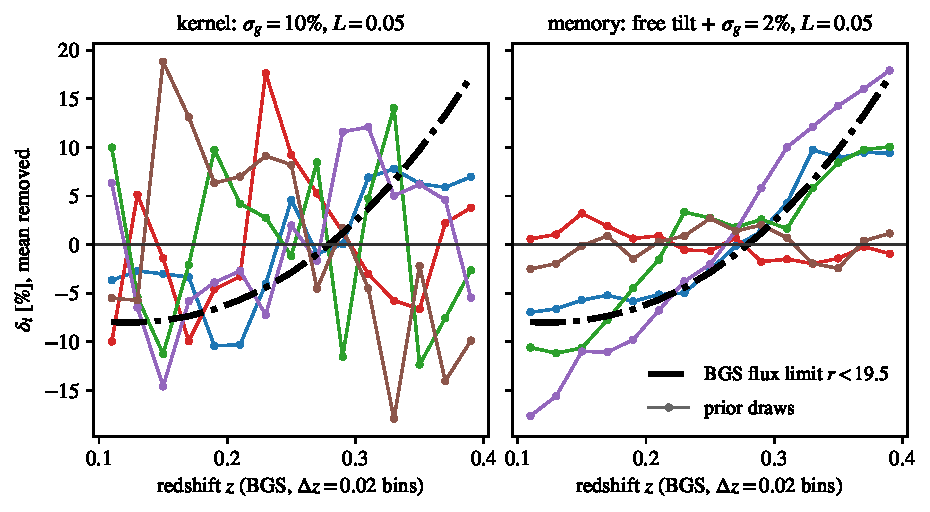
\includegraphics[width=\linewidth]{plots/theory_draws/theory_draws.pdf}
  \caption{Random prior draws of the deviations of the 15 BGS bins at
    $\Delta z = 0.02$, each draw's mean removed ($B_g$ is free).  Thick
    dash-dot: the BGS flux-limit drift.  Left: the kernel model.
    Right: the memory model, whose tilt is free in the model and drawn
    here, for display only, from a Gaussian of width $0.6$ per unit
    redshift.}
  \label{fig:theorydraws}
\end{figure}

\subsection{Why the memory model differs physically}
\label{sec:memphysics}

A selected sample changes along a group in two ways.  Coherent changes
move every bin the same way: a threshold that rises with distance, the
debiasing of a conserved population.  Local changes move bins
independently and are forgotten over a short range: the sky-line
windows and filter-edge crossings of Appendix~\ref{sec:selection}.  The
memory model gives the first kind to the tilt and the second to the
kernel.  One line suffices for the coherent kind, because the drifts
are smooth functions of $D(z)$ and the distance modulus.  The best
equal-weight line through each group's conserved deviation at the
$\Delta z = 0.05$ bin centers (derived; amplitudes $1.34$ for BGS,
$1.70$ for the LRGs and $0.84$ for the ELGs) removes deviations that
span $3$--$11\%$ and leaves $0.02$--$0.16\%$ rms, at most $0.27\%$
(ELG2).  The BGS flux-limit drift is larger and convex: it spans
$22.3\%$, and its best line leaves $2.4\%$ rms and $3.3\%$ at most
(Appendix~\ref{app:bgsflux}).  Figure~\ref{fig:theorydelta} shows both.
In the memory model $\sigma_g$ is the departure from the group's own
line, curvature plus local scatter: about $0.1\%$ for a conserved
population, $1$--$2\%$ for local selection features, $2$--$3\%$ for the
BGS curvature.

\begin{figure}[htbp]
  \centering
  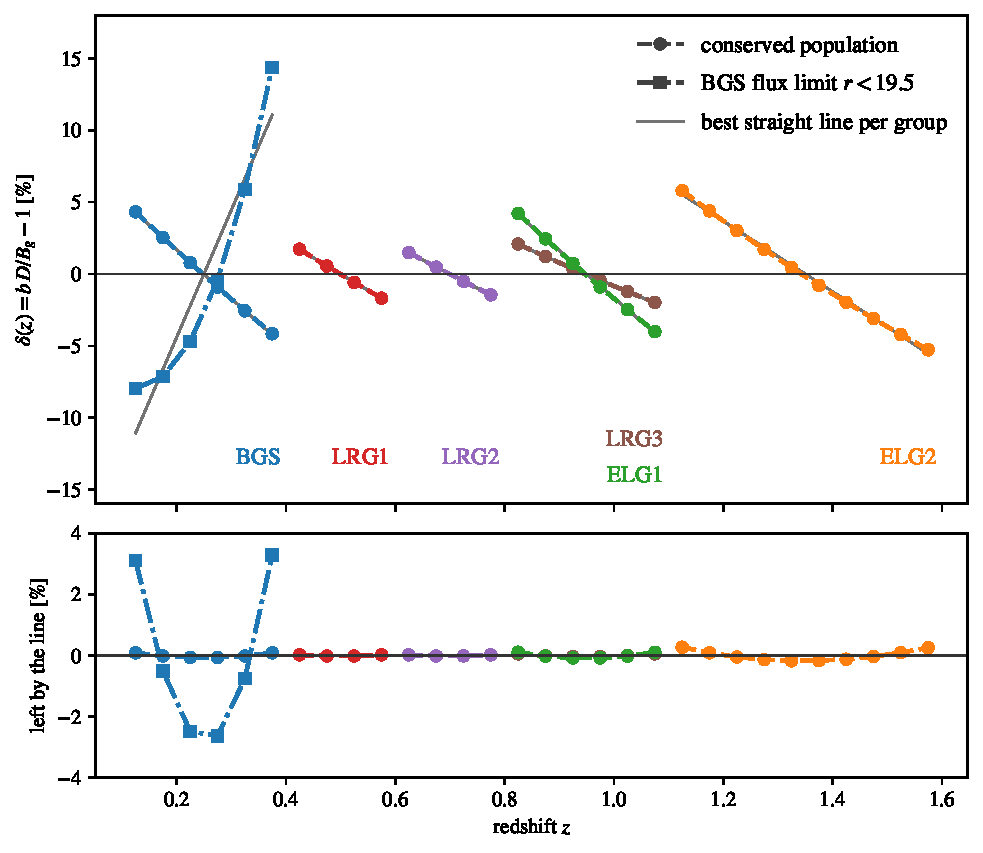
\includegraphics[width=\linewidth]{plots/theory_delta/theory_delta.pdf}
  \caption{Top: the deviation $\delta(z) = b\,D/B_g - 1$ at the
    $\Delta z = 0.05$ bin centers, with $B_g$ set so the mean deviation
    vanishes.  Dashed with circles: the conserved population, every
    group.  Dash-dot with squares: the BGS flux limit.  Thin gray: the
    best straight line per curve.  Bottom: what the line leaves.}
  \label{fig:theorydelta}
\end{figure}

\subsection{What the prior charges}
\label{sec:memcharge}

With flat priors on the line's level and slope, the prior precision of
a group's bin amplitudes is (Appendix~\ref{app:memory})
\begin{equation}
  \Prec_{\rm mem}
  \;=\;
  \mathsf{Q} - \mathsf{Q}\,\mathsf{U}
  \bigl(\mathsf{U}\T \mathsf{Q}\, \mathsf{U}\bigr)^{-1}
  \mathsf{U}\T \mathsf{Q},
  \qquad
  \mathsf{Q} = \Cov^{-1},
  \qquad
  \mathsf{U} = [\,\ones,\ v\,],
  \label{eq:memproj}
\end{equation}
the construction of Eq.~\eqref{eq:projdef} with one more column.  Its
penalty is
\begin{equation}
  \delta\T \Prec_{\rm mem}\, \delta
  \;=\;
  \min_{c,\, s_g}\;
  \bigl(\delta - c\,\ones - s_g\, v\bigr)\T
  \mathsf{Q}
  \bigl(\delta - c\,\ones - s_g\, v\bigr) :
  \label{eq:memmin}
\end{equation}
the prior subtracts the best straight line and charges only the
residual.  A monotonic drift of any size costs nothing; bumps around
the line still cost, and still forget over $L$.  $\mathsf{Q}$ is
tridiagonal (Appendix~\ref{sec:general}), while the subtracted term has
rank two and is dense, because the fitted line listens to every bin.
$\Prec_{\rm mem}\mathsf{U} = 0$, $\Prec_{\rm mem}$ is positive
semidefinite with rank $n - 2$, and a group of one or two bins has
$\Prec_{\rm mem} = 0$.

\section{The bias continuity equation, step by step}
\label{app:continuity}

The matter overdensity is $\delta_m = (\rho_m - \bar\rho_m)/\bar\rho_m$,
with $\bar\rho_m(t)$ the mean density; the galaxy-count overdensity
$\delta_{\rm gal}$ is defined the same way.  Conservation of mass and of
galaxy number gives, in comoving coordinates and to linear order (the
convective term $\mathbf{v} \cdot \nabla \delta$ is second order),
\begin{equation}
  \frac{\partial \delta_m}{\partial t}
  \;=\;
  -\,\frac{1}{a}\,\nabla \cdot \mathbf{v}_m,
  \qquad
  \frac{\partial \delta_{\rm gal}}{\partial t}
  \;=\;
  -\,\frac{1}{a}\,\nabla \cdot \mathbf{v}_{\rm gal},
  \label{eq:continuity}
\end{equation}
with $t$ cosmic time and $\mathbf{v}_m$, $\mathbf{v}_{\rm gal}$ the
peculiar velocities.  On large scales galaxies fall in the same
potential as the matter and carry no pressure of their own, so
$\mathbf{v}_{\rm gal} = \mathbf{v}_m$ (no velocity bias; galaxies as
test particles in Tegmark and Peebles~\cite{TegmarkPeebles1998}).
Subtracting the two equations and integrating from $z_c$,
\begin{equation}
  \delta_{\rm gal}(z) - \delta_m(z)
  \;=\;
  \delta_{\rm gal}(z_c) - \delta_m(z_c) :
  \label{eq:frozen}
\end{equation}
the excess clumping keeps its initial value.  With
$\delta_{\rm gal}(z_c) = b_c\,\delta_m(z_c)$ and
$\delta_m(z) = \delta_m(z_c)\, D(z)/D(z_c)$,
\begin{equation}
  \delta_{\rm gal}(z)
  \;=\;
  \delta_m(z)
  \left[\,1 + \bigl(b_c - 1\bigr)\,\frac{D(z_c)}{D(z)}\,\right],
  \label{eq:appsub}
\end{equation}
and dividing by $\delta_m(z)$ gives Eq.~\eqref{eq:fry}; dividing by the
growth-tied bias gives Eq.~\eqref{eq:tilt}.  As $D$ grows the frozen
term is divided by an ever larger number, so $b \to 1$: gravity
debiases a conserved sample.

Tegmark and Peebles also allow stochastic bias, with $b$ the ratio of
the galaxy to the matter fluctuation amplitude and $\rho_{gm}$ the
correlation coefficient of the two fields.  The same argument evolves
both: with $D$ normalized to one today and the subscript zero marking
today,
\begin{equation}
  b_0 =
  \left[(1 - D)^2 + 2 D (1 - D)\, b\, \rho_{gm}
  + D^2 b^2\right]^{1/2},
  \qquad
  \rho_{gm,0} = \frac{(1 - D) + D\, b\, \rho_{gm}}{b_0},
  \label{eq:tpevol}
\end{equation}
with $b$ and $\rho_{gm}$ the values at the epoch of growth factor $D$.
Both approach one as clustering grows, and for $\rho_{gm} = 1$
Eq.~\eqref{eq:tpevol} collapses to $b_0 - 1 = (b - 1)\,D$,
Eq.~\eqref{eq:fry} again.  For a DESI sample the assumption that
breaks is conservation (Appendix~\ref{sec:selection}); no velocity
bias and linear theory hold well on the scales kept.  The script of
Appendix~\ref{app:verify} integrates Eq.~\eqref{eq:continuity} and
recovers Eq.~\eqref{eq:fry} to $2 \times 10^{-9}$.

\section{The BGS flux-limit bias model, step by step}
\label{app:bgsflux}

This appendix derives the BGS drift of the baseline prior: a $22.3\%$
span, a convex shape, and a $2.4\%$ rms residual around the best line
(the function \texttt{bgs\_flux\_limit\_bias} of
\texttt{plots/make\_theory\_data.py}).

\subsection{The four steps}
\label{sec:bgssteps}

\paragraph{Step 1: the flux limit becomes a luminosity threshold.}
BGS Bright keeps every galaxy brighter than $r = 19.5$~\cite{Hahn2023}
($r$ the magnitude band).  The apparent magnitude $r$ and the absolute
magnitude $M$ are related by
$r = M + 25 + 5\log_{10}[d_L/(h^{-1}\,{\rm Mpc})] + K(z)$, with $d_L$
the luminosity distance and $K(z)$ the K-correction, the magnitude
correction for the part of the redshifted spectrum that falls outside
the observed band~\cite{BlantonRoweis2007}.  With $K = 0$ the faintest
absolute magnitude that passes at redshift $z$ is
\begin{equation}
  M_{\rm lim}(z) - 5\log_{10} h
  \;=\;
  19.5 - 25 - 5\log_{10} \frac{d_L(z)}{h^{-1}\,{\rm Mpc}},
  \qquad
  d_L(z) \;=\; (1+z)\,\chi(z),
  \label{eq:bgsmlim}
\end{equation}
with $\chi(z)$ the comoving distance of flat $\Lambda$CDM with
$\Omega_m = 0.3$ and $h$ the Hubble constant in units of
$100$~km/s/Mpc.

\paragraph{Steps 2 and 3: each bin is a threshold sample, and the
threshold sets the bias.}
At redshift $z$ the sample holds every galaxy with
$M < M_{\rm lim}(z)$, a threshold that brightens with distance.  The
SDSS luminosity-threshold samples at $z < 0.25$~\cite{Zehavi2011}
give
\begin{equation}
  b(>L_{\rm th})
  \;=\;
  1.06 + 0.21\,(L_{\rm th}/L_*)^{1.12},
  \qquad
  L_{\rm th}/L_* \;=\; 10^{-0.4\,(M_{\rm lim} - M_*)},
  \label{eq:bgszehavi}
\end{equation}
with $M_* - 5\log_{10} h = -20.44$ the characteristic magnitude of the
SDSS $r$-band luminosity function~\cite{Blanton2003}.  The model
applies the fit at every redshift, without evolution, and reads the
published $b\,(\sigma_8/0.8)$ as $b$.

\paragraph{Step 4: the deviation from the growth-tied shape.}
Because $B_g$ is free, only the shape of $b(z)$ matters; the amplitude
makes the mean deviation over the group's bin centers vanish:
\begin{equation}
  \delta(\bar{z}_i)
  \;=\;
  \frac{b(\bar{z}_i)\,D(\bar{z}_i)}{B} - 1,
  \qquad
  B \;=\; \frac{1}{n}\sum_{j=1}^{n} b(\bar{z}_j)\,D(\bar{z}_j).
  \label{eq:bgsdelta}
\end{equation}
At the six $\Delta z = 0.05$ bin centers of BGS, $z = 0.125$ to
$0.375$, the threshold brightens from $-18.56$ to $-21.24$, so
$L_{\rm th}/L_*$ grows from $0.18$ to $2.10$ and the bias from $1.09$
to $1.54$, while $D$ falls from $0.937$ to $0.824$.  The deviation runs
from $-8.0\%$ to $+14.4\%$, the $22.3\%$ span of
Figure~\ref{fig:theorydelta}.

\subsection{Why the drift is convex}
\label{sec:bgsconvex}

The bias rises by $41\%$ while $D$ falls by $12\%$, so the deviation
inherits the shape of the bias curve, which is flat at low redshift
and steep at high redshift: below $L_*$ the term
$0.21\,(L_{\rm th}/L_*)^{1.12}$ is small against $1.06$ ($0.03$ at the
first center), the threshold crosses $L_*$ near $z = 0.27$, and beyond
it the term rises exponentially ($0.48$ at the last center).  A
straight line through a convex curve leaves a U-shaped residual,
$(+3.1, -0.5, -2.5, -2.6, -0.8, +3.3)\%$ here.  Adding a quadratic term
cuts the residual from $2.4\%$ to $0.1\%$ rms, so the $2.4\%$ is the
curvature of the drift, the one part a free tilt cannot absorb.

\subsection{What the model leaves out}
\label{sec:bgsomissions}

None of the omissions changes the qualitative shape, a smooth,
monotonic, convex rise toward the far edge of the group.
\begin{itemize}
  \item \textbf{Evolution of the threshold-bias relation.}  The bias at
    fixed luminosity grows with redshift (Eq.~\eqref{eq:fry}), which
    steepens the drift; $M_*$ brightens by $1$--$2$ magnitudes per unit
    redshift~\cite{Blanton2003}, which flattens it, but only by
    $0.3$--$0.6$ magnitudes at the last center against the $2.68$ of
    the threshold.
  \item \textbf{No K-correction.}  A positive $K$, $0.37$ magnitudes at
    $z = 0.4$ for a spectrum flat in wavelength and more for a red
    one~\cite{BlantonRoweis2007}, makes the true threshold brighter at
    high redshift and steepens the drift.
  \item \textbf{Only $r < 19.5$.}  BGS Faint, at
    $19.5 < r < 20.175$~\cite{Hahn2023}, lowers the threshold by $0.675$
    magnitudes and flattens the drift; the fiber-magnitude cut and the
    color selection change the galaxy mix in a way
    Eq.~\eqref{eq:bgszehavi} cannot follow.
\end{itemize}
The model is an order-of-magnitude estimate, not a prediction of the
measured DESI BGS bias.  Its reliable content is the shape of the drift
and its size to a factor of order unity, which is what the baseline
prior uses: $\sigma_g = 3\%$ for BGS, from the $2$--$3\%$ curvature.
 right after \appendix.  No preamble: the
% macros \ones, \Prec, \Cov and \T come from the main file.  The labels
% are shared with the mathematics appendices (appendix_math.tex).

\section{The models}
\label{sec:models}

This appendix first builds the prior without the tilt of
Eq.~\eqref{eq:summodel}: the kernel model, in which the exponential
kernel describes the whole deviation $\delta_i$ of a bin from its
group's trend.  Appendix~\ref{sec:memory} adds the free tilt, and the
kernel then describes the residual $\varepsilon_i$ around each group's
line.  In the appendices $b_i$ is the linear bias $b_{1,i}$ of bin $i$.

\subsection{Growth-tied, free, and correlated biases}
\label{sec:defs}

The growth-tied model sets $b_i = B_g/D(\bar{z}_i)$, with one free
amplitude $B_g$ per group.  The kernel model multiplies it by a
fractional deviation $\delta_i$,
\begin{align}
  b_i &\;=\; \frac{B_g}{D(\bar{z}_i)}\,\bigl(1 + \delta_i\bigr),
  \label{eq:model}
  \\
  \bigl\langle \delta_i\,\delta_j \bigr\rangle
  &\;=\; \sigma_g^2\,
  \exp\!\left(-\,\frac{|\bar{z}_i - \bar{z}_j|}{L}\right),
  \label{eq:priorkernel}
\end{align}
with $B_g$ still free (flat prior) and the prior zero across groups.
In the Fisher matrix the convenient parameters are the per-bin
amplitudes
\begin{equation}
  \beta_i \;\equiv\; B_g\,\bigl(1 + \delta_i\bigr),
  \qquad \text{fiducial } \beta_i = B_g,
  \label{eq:beta}
\end{equation}
so that $b_i = \beta_i / D(\bar{z}_i)$.  Since
$\beta_i - B_g = B_g\,\delta_i$, the prior covariance of the $\beta_i$
within one group is
\begin{equation}
  \Cov \;=\; \sigma_\beta^2\,\mathsf{R},
  \qquad
  \sigma_\beta \;=\; \sigma_g\,B_g,
  \qquad
  \mathsf{R}_{ij} \;=\; \exp\!\left(-\,\frac{|\bar{z}_i - \bar{z}_j|}{L}\right),
  \label{eq:covdef}
\end{equation}
with $\sigma_\beta$ the spread of one amplitude, in units of a bias, and
$\mathsf{R}$ the dimensionless correlation matrix.

\subsection{What $\sigma_g$ and $L$ mean}
\label{sec:jump}

The diagonal of the kernel gives the wander of a single bin,
$\mathrm{Var}(\delta_i) = \sigma_g^2$.  The correlation coefficient of
two bins at separation $\Delta z = |\bar{z}_i - \bar{z}_j|$ is
\begin{equation}
  r \;=\;
  \frac{\langle \delta_i \delta_j \rangle}
       {\sqrt{\langle \delta_i^2 \rangle\,\langle \delta_j^2 \rangle}}
  \;=\; e^{-\Delta z / L} ,
  \label{eq:rdef}
\end{equation}
set by the separation and $L$ alone.  The jump between the two bins has
variance
\begin{equation}
  \mathrm{Var}(\delta_i - \delta_j)
  \;=\;
  2\,\sigma_g^2\left(1 - e^{-\Delta z / L}\right)
  \;\approx\;
  \frac{2\,\sigma_g^2\,\Delta z}{L}
  \quad (\Delta z \ll L).
  \label{eq:jumpvar}
\end{equation}
At small separations the jump variance grows linearly with
$\Delta z$, as for a random walk; only beyond $L$ does the finite
wander pull the deviation back.  For neighbors at $\Delta z = 0.02$
with $L = 0.05$, $r = e^{-0.4} = 0.670$ and the exact rms jump is
$0.81\,\sigma_g$; the small-separation form gives $0.89\,\sigma_g$,
because $\Delta z/L = 0.4$ is not small.

\subsection{The free group amplitude and the projection}
\label{sec:projintro}

A plain Gaussian prior with covariance $\Cov$ would charge for moving
all $\beta_i$ of a group together, but that uniform shift is the free
amplitude $B_g$.  The repair removes the uniform direction: with
$\ones$ the ones vector of the group's $n$ bins, the prior precision
of a group's amplitudes is
\begin{equation}
  \Prec \;=\; \Cov^{-1}
  \;-\;
  \frac{\Cov^{-1}\ones\,\ones\T \Cov^{-1}}{\ones\T \Cov^{-1} \ones}.
  \label{eq:projdef}
\end{equation}
$\Prec\,\ones = 0$, so a uniform shift costs nothing; a pure shape
change keeps the penalty of the plain prior; $\Prec$ is positive
semidefinite (no displacement has a negative penalty) with rank
$n - 1$; and $\Prec$ is exactly the prior
obtained by sampling $B_g$ with a flat prior and marginalizing it.
Appendices~\ref{sec:twobins}, \ref{sec:threeviews} and
\ref{sec:general} show these for two bins, by marginalization, and for
$n$ bins.  Across groups the prior is zero, so the full prior
precision is block diagonal.

\section{Which $L$ and $\sigma_g$ are physical}
\label{sec:physical}

One case of bias evolution can be solved in closed form: a population
whose members are conserved.  This appendix derives it, measures its
deviation from the growth-tied trend, lists what breaks conservation in
a selected sample, and weighs the published measurements.

\subsection{A conserved population: the bias continuity equation}
\label{sec:conserved}

Take a sample whose membership never changes, with no velocity bias,
in linear theory.  The matter overdensity $\delta_m$ and the
galaxy-count overdensity $\delta_{\rm gal}$ then obey the same
continuity equation with the same velocity field, so the excess
clumping $\delta_{\rm gal} - \delta_m$ is frozen
(Appendix~\ref{app:continuity}).  With $b_c$ the linear bias at a
reference redshift $z_c$ and $\delta_m \propto D$, the frozen
difference gives~\cite{Fry1996}
\begin{equation}
  b(z) - 1
  \;=\;
  \bigl(b_c - 1\bigr)\,\frac{D(z_c)}{D(z)} :
  \label{eq:fry}
\end{equation}
the excess set at formation stays fixed while the matter clustering
grows, so the bias decays toward one.  The growth-tied shape freezes a
different quantity: constant $b\,D$ means a galaxy clustering amplitude
$b\,\delta_m$ that does not grow, which describes a selection that
picks, at each redshift, a different and rarer set of objects.

\subsection{The deviation from the growth-tied trend}
\label{sec:tilt}

Place the reference at a group's midpoint $z_c$, with
$b_c = B/D(z_c)$.  The ratio of Eq.~\eqref{eq:fry} to the growth-tied
bias $b_c\,D(z_c)/D(z)$ gives the deviation of Eq.~\eqref{eq:model},
\begin{equation}
  \delta(z)
  \;=\;
  \frac{D(z)/D(z_c) - 1}{b_c} ,
  \label{eq:tilt}
\end{equation}
zero at the midpoint, positive at lower redshift and negative at higher
redshift, and nearly linear across a group because $D$ is smooth.  In
flat $\Lambda$CDM with $\Omega_m = 0.3$ and the project's fiducial
amplitudes it is $+5.3\%$ and $-4.9\%$ at the ends of BGS ($B = 1.34$,
$0.1 < z < 0.4$, $b_c = 1.5$), $+2.4\%$ and $-2.2\%$ at the ends of LRG1
($B = 1.70$, $0.4 < z < 0.6$, $b_c = 2.2$), and $+2.6\%$ and $-2.3\%$ at
the ends of LRG3 ($B = 1.70$, $0.8 < z < 1.1$, $b_c = 2.7$).  Between
neighbors it changes by $0.3$--$0.7\%$ at $\Delta z = 0.02$ and
$0.8$--$1.7\%$ at $\Delta z = 0.05$: a smooth tilt, coherent over the
whole group.  For comparison, the neighbor rms of
Eq.~\eqref{eq:jumpvar} at $\Delta z = 0.02$ (and $0.05$) is $2.4\%$
($3.4\%$) for $\sigma_g = 3\%$ and $L = 0.05$, and $0.44\%$ ($0.67\%$)
for $\sigma_g = 1\%$ and $L = 0.2$.  Figure~\ref{fig:theorybz} draws
these shapes: the conserved curve is flatter than $B_g/D$ in every
group, while the BGS flux-limit curve is much steeper, and convex.

\begin{figure}[htbp]
  \centering
  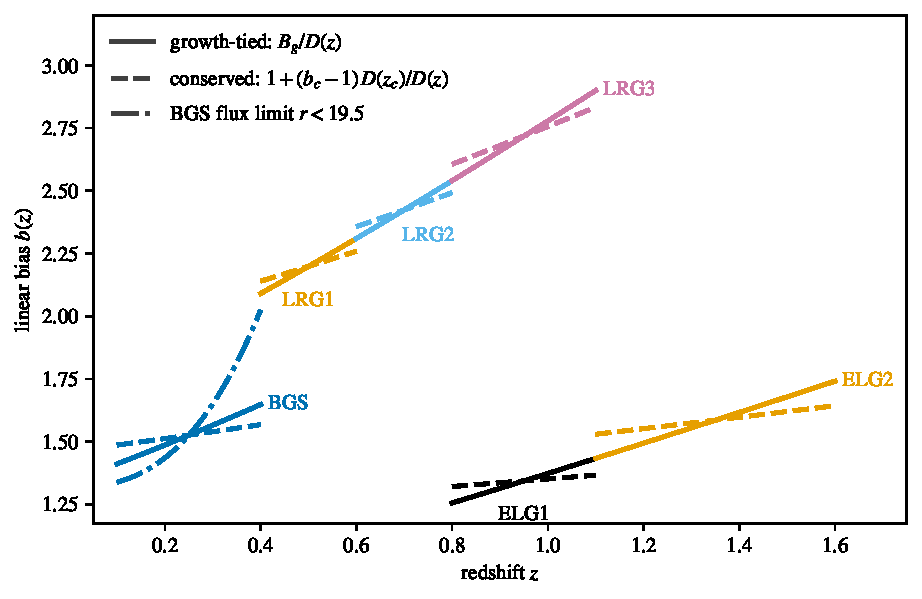
\includegraphics[width=\linewidth]{plots/theory_bz/theory_bz.pdf}
  \caption{The bias $b(z)$ of every group.  Solid: the growth-tied
    shape $B_g/D(z)$.  Dashed: a conserved population anchored at the
    group midpoint (Eq.~\eqref{eq:fry}).  Dash-dot, on BGS only: the
    $r < 19.5$ flux-limit bias, anchored at the same midpoint.}
  \label{fig:theorybz}
\end{figure}

\subsection{What breaks conservation in a selected sample}
\label{sec:selection}

\begin{itemize}
  \item \textbf{Threshold drift.}  A selection holds a roughly constant
    comoving density until the flux limit bites; beyond, it keeps only
    its brighter, more biased members.  The change is smooth, with $L$
    comparable to the group width.
  \item \textbf{Color-selection features.}  A spectral feature crossing
    a filter edge moves a color cut quickly in redshift.  The sharpest
    is the $4000$~\AA\ break, the step in an old galaxy's rest-frame
    spectrum at $4000$~\AA, which redshift slides across the filters: a
    filter edge $100$--$200$~\AA\ wide maps to
    $\Delta z = \Delta\lambda/(4000~\text{\AA}) \approx 0.03$--$0.05$.  The crossing is known; its
    amplitude in bias is unmeasured.
  \item \textbf{Mergers} turn two members into one.
  \item \textbf{Emission-line selection.}  An ELG belongs to the sample
    while its lines are strong, so membership follows the
    star-formation phase.
\end{itemize}

\subsection{What the measurements say}
\label{sec:evidence}

Each statement is tagged \emph{measured} (read from the cited source),
\emph{derived} (computed here from measured inputs) or \emph{assumed}.
Equation~\eqref{eq:fry} is from Fry~\cite{Fry1996};
Tegmark and Peebles~\cite{TegmarkPeebles1998} rederive it.

\paragraph{Massive red galaxies follow the conserved shape.}
SDSS and 2SLAQ LRGs at $0.19 < z < 0.55$, matched in color and
luminosity, show no significant evolution of the clustering amplitude
and merge at $7.5 \pm 2.3\%$ over that range, about $2.4\%$ per
Gyr~\cite{Wake2008} (measured).  The BOSS progenitors of the SDSS LRGs
merge at $2 \pm 1.5\%$ per Gyr and cluster as the continuity equation
predicts~\cite{Tojeiro2012}, and CMASS samples of fixed comoving
density at $0.43 < z < 0.7$ cluster like a conserved
population~\cite{Guo2013} (measured).  The bias of DESI-like LRGs in
photometric bins of $\Delta z \approx 0.1$ stays within $\pm 2.3\%$ of
$b = 1.5/D$ below $z = 0.83$, with the highest bin $6.4 \pm 6.4\%$
high~\cite{Zhou2021} (measured biases, residuals derived;
Figure~\ref{fig:zhou}).

\begin{figure}[htbp]
  \centering
  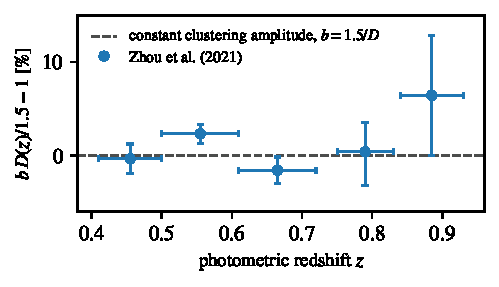
\includegraphics{plots/zhou_lrg_bias/zhou_lrg_bias.pdf}
  \caption{The measured bias of DESI-like LRGs~\cite{Zhou2021} as a
    fractional residual around $b = 1.5/D$, with $D$ at each
    photometric bin's center (flat $\Lambda$CDM, $\Omega_m = 0.3$);
    horizontal bars: the bin edges.}
  \label{fig:zhou}
\end{figure}

\paragraph{The selections drift.}
The DESI LRG cuts hold the comoving density near
$5 \times 10^{-4}\,(h/{\rm Mpc})^3$ at $0.4 < z < 0.8$ and hand over to
a fixed flux limit beyond~\cite{Zhou2023lrg} (measured).  That limit
raises the luminosity threshold by $0.27$ magnitudes per
$\Delta z = 0.1$ at $z \approx 1$; times the threshold-bias slope of
SDSS luminosity-threshold samples, $b\,(\sigma_8/0.8) = 1.06 +
0.21\,(L_{\rm th}/L_*)^{1.12}$~\cite{Zehavi2011} ($0.5$--$1.0$ in bias
per magnitude near LRG luminosities; measured), it drifts the LRG3 bias
by $6$--$11\%$ per $\Delta z = 0.1$ on top of $B/D$ (derived, from an
$r$-band relation outside its calibrated range, so only the direction
and order of magnitude hold).  BGS Bright is magnitude limited at
$r < 19.5$~\cite{Hahn2023} (measured), which drives a $10$--$25\%$ bias
drift across the group (derived; Appendix~\ref{app:bgsflux}).

\paragraph{The ELG bias shape is stable.}
Fits of the halo occupation distribution (HOD: how many sample
galaxies live in a halo of each mass) to the DESI One-Percent ELGs in
$0.8 < z < 1.1$ and
$1.1 < z < 1.6$ agree within one sigma~\cite{Rocher2023} (measured);
at these host masses the halo bias depends weakly on mass, so the
implied drift is at the percent level (derived, slope assumed).  The
[OII] doublet loses signal-to-noise in windows
$\Delta z \approx 0.001$--$0.01$ wide where it lands on sky lines,
especially at $z > 1.5$~\cite{Raichoor2023} (measured): the one
short-separation mechanism with a measured location, with an assumed
bias amplitude of $1$--$2\%$.

\paragraph{Nothing resolves bias below $\Delta z \approx 0.1$.}
The CMB-lensing tomography of the same samples~\cite{White2022,
Sailer2024, Sailer2025}, on the photometric samples of
Zhou et al.~\cite{Zhou2023tomo}, uses bins of about $0.15$ with one
free bias per bin and finds smooth models that fit.  Below
$\Delta z \approx 0.1$ this note rests on the continuity equation and
the selection arguments.

\section{The memory model}
\label{sec:memory}

\subsection{Why a second model}
\label{sec:memwhy}

Every deviation above except the sky-line windows is a monotonic drift:
the conserved-population tilt (about $1\%$ per $\Delta z = 0.05$), the
LRG3 magnitude-limit drift ($6$--$11\%$ per $\Delta z = 0.1$) and the
BGS flux-limit drift ($10$--$25\%$ across the group).  The kernel model
admits such a drift only at a price: to pass a $20\%$ drift with
$L \leq 0.1$ it takes $\sigma_g = 10$--$15\%$, which also allows about
$10\%$ scatter between neighbors that no identified mechanism
produces.  One $\sigma_g$ controls both, so the kernel cannot say
``large smooth drift, small local scatter''.  The memory model
separates the two.

\subsection{Why the kernel forgets}
\label{sec:memforget}

At $L = 0.05$, bins $0.15$ apart share $e^{-3} \approx 0.05$ of their
deviation.  With $r_k = e^{-(\bar{z}_{k+1} - \bar{z}_k)/L}$ the
correlation of neighbors $k$ and $k+1$, the best guess of the next bin
given all earlier ones is (Appendix~\ref{app:chain})
\begin{equation}
  \mathrm{E}\bigl[\delta_{k+1} \mid \delta_1, \dots, \delta_k\bigr]
  \;=\; r_k\, \delta_k :
  \label{eq:memmarkov}
\end{equation}
only the nearest neighbor matters, and the influence of any one bin
fades along the chain.

\subsection{The model, and why it remembers}
\label{sec:memmodel}

The memory model adds a tilt per group and splits the deviation into a
line and a residual,
\begin{equation}
  \delta_i \;=\; s_g\, v_i + \varepsilon_i,
  \qquad
  v_i \;=\; \bar{z}_i - \bar{z}_g,
  \label{eq:memdef}
\end{equation}
with $s_g$ a free tilt (flat prior, like $B_g$) and $\varepsilon_i$
carrying the kernel of Eq.~\eqref{eq:priorkernel}: the model of
Eqs.~\eqref{eq:summodel} and \eqref{eq:sumkernel}.  Giving the slope a
Gaussian prior of variance $\tau^2$ first (the flat prior is
$\tau \to \infty$), the deviations have covariance
\begin{equation}
  \mathrm{Cov}(\delta_i, \delta_j)
  \;=\;
  \tau^2\, v_i\, v_j
  \;+\;
  \sigma_g^2\, e^{-|\bar{z}_i - \bar{z}_j|/L} .
  \label{eq:memcov}
\end{equation}
The new term does not decay with separation.  Far beyond $L$ the
correlation coefficient tends to
\begin{equation}
  \rho_{ij}
  \;\longrightarrow\;
  \frac{\tau^2 v_i v_j}
       {\sqrt{\bigl(\tau^2 v_i^2 + \sigma_g^2\bigr)
              \bigl(\tau^2 v_j^2 + \sigma_g^2\bigr)}}
  \;\longrightarrow\; \pm 1
  \quad \text{when } \tau |v| \gg \sigma_g :
  \label{eq:memrho}
\end{equation}
the two ends of a group remember each other through the shared slope.
The best guess of the next bin becomes
\begin{equation}
  \mathrm{E}\bigl[\delta_{k+1} \mid \delta_1, \dots, \delta_k\bigr]
  \;=\;
  \hat{c} + \hat{s}_g\, v_{k+1}
  \;+\;
  r_k\,\bigl(\delta_k - \hat{c} - \hat{s}_g\, v_k\bigr),
  \label{eq:memkriging}
\end{equation}
with $(\hat{c}, \hat{s}_g)$ the level and slope of the best straight
line through all past bins, weighted by $\Cov^{-1}$: every past bin
enters through the fitted line, and only the wiggle around it stays
Markov (the universal-kriging predictor; kriging is the geostatistics
name for the best linear prediction from correlated data;
Appendix~\ref{app:memory}).
Figure~\ref{fig:theorydraws} shows the difference on the BGS bins at
$\Delta z = 0.02$: kernel draws wide enough to admit the BGS drift
zigzag and forget, while memory draws are lines with small wiggles,
among which the drift looks typical.

\begin{figure}[htbp]
  \centering
  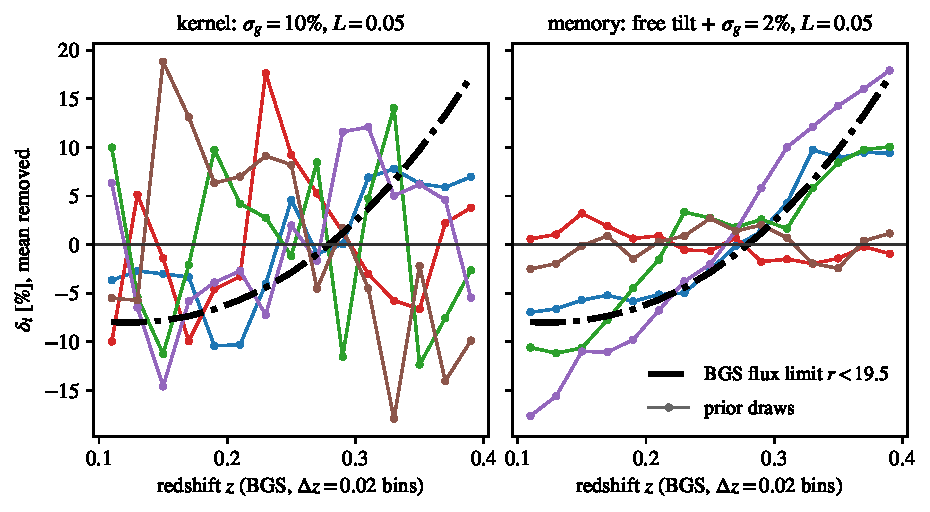
\includegraphics[width=\linewidth]{plots/theory_draws/theory_draws.pdf}
  \caption{Random prior draws of the deviations of the 15 BGS bins at
    $\Delta z = 0.02$, each draw's mean removed ($B_g$ is free).  Thick
    dash-dot: the BGS flux-limit drift.  Left: the kernel model.
    Right: the memory model, whose tilt is free in the model and drawn
    here, for display only, from a Gaussian of width $0.6$ per unit
    redshift.}
  \label{fig:theorydraws}
\end{figure}

\subsection{Why the memory model differs physically}
\label{sec:memphysics}

A selected sample changes along a group in two ways.  Coherent changes
move every bin the same way: a threshold that rises with distance, the
debiasing of a conserved population.  Local changes move bins
independently and are forgotten over a short range: the sky-line
windows and filter-edge crossings of Appendix~\ref{sec:selection}.  The
memory model gives the first kind to the tilt and the second to the
kernel.  One line suffices for the coherent kind, because the drifts
are smooth functions of $D(z)$ and the distance modulus.  The best
equal-weight line through each group's conserved deviation at the
$\Delta z = 0.05$ bin centers (derived; amplitudes $1.34$ for BGS,
$1.70$ for the LRGs and $0.84$ for the ELGs) removes deviations that
span $3$--$11\%$ and leaves $0.02$--$0.16\%$ rms, at most $0.27\%$
(ELG2).  The BGS flux-limit drift is larger and convex: it spans
$22.3\%$, and its best line leaves $2.4\%$ rms and $3.3\%$ at most
(Appendix~\ref{app:bgsflux}).  Figure~\ref{fig:theorydelta} shows both.
In the memory model $\sigma_g$ is the departure from the group's own
line, curvature plus local scatter: about $0.1\%$ for a conserved
population, $1$--$2\%$ for local selection features, $2$--$3\%$ for the
BGS curvature.

\begin{figure}[htbp]
  \centering
  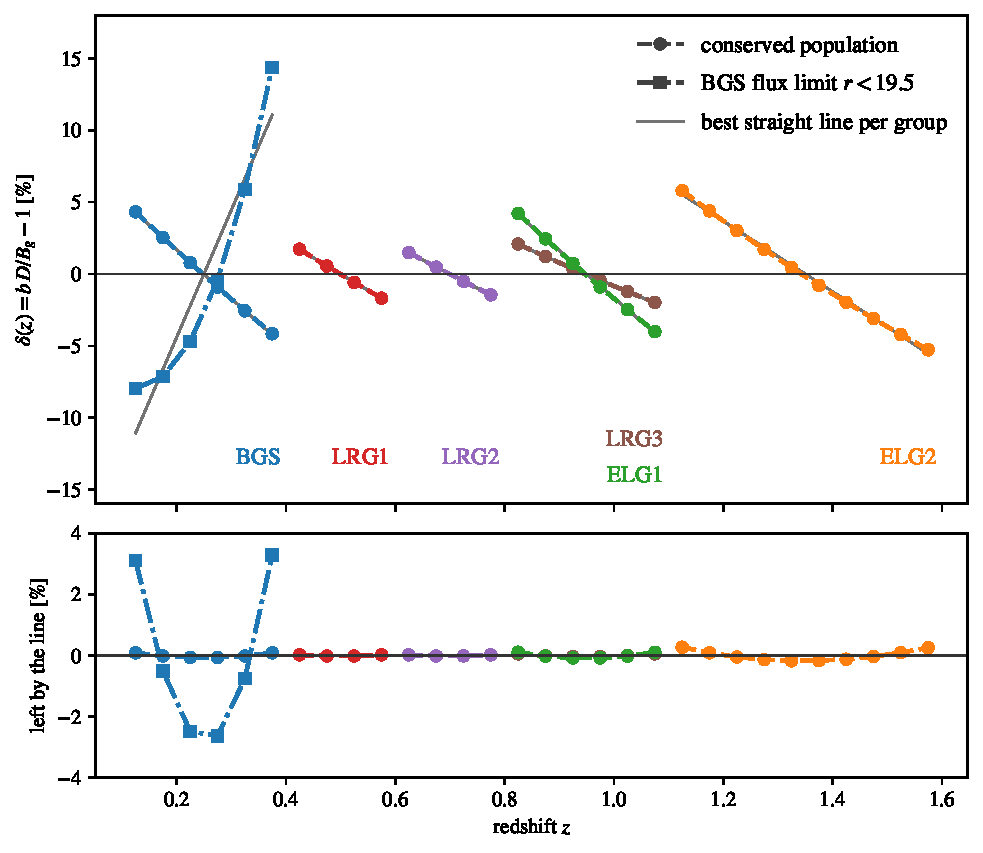
\includegraphics[width=\linewidth]{plots/theory_delta/theory_delta.pdf}
  \caption{Top: the deviation $\delta(z) = b\,D/B_g - 1$ at the
    $\Delta z = 0.05$ bin centers, with $B_g$ set so the mean deviation
    vanishes.  Dashed with circles: the conserved population, every
    group.  Dash-dot with squares: the BGS flux limit.  Thin gray: the
    best straight line per curve.  Bottom: what the line leaves.}
  \label{fig:theorydelta}
\end{figure}

\subsection{What the prior charges}
\label{sec:memcharge}

With flat priors on the line's level and slope, the prior precision of
a group's bin amplitudes is (Appendix~\ref{app:memory})
\begin{equation}
  \Prec_{\rm mem}
  \;=\;
  \mathsf{Q} - \mathsf{Q}\,\mathsf{U}
  \bigl(\mathsf{U}\T \mathsf{Q}\, \mathsf{U}\bigr)^{-1}
  \mathsf{U}\T \mathsf{Q},
  \qquad
  \mathsf{Q} = \Cov^{-1},
  \qquad
  \mathsf{U} = [\,\ones,\ v\,],
  \label{eq:memproj}
\end{equation}
the construction of Eq.~\eqref{eq:projdef} with one more column.  Its
penalty is
\begin{equation}
  \delta\T \Prec_{\rm mem}\, \delta
  \;=\;
  \min_{c,\, s_g}\;
  \bigl(\delta - c\,\ones - s_g\, v\bigr)\T
  \mathsf{Q}
  \bigl(\delta - c\,\ones - s_g\, v\bigr) :
  \label{eq:memmin}
\end{equation}
the prior subtracts the best straight line and charges only the
residual.  A monotonic drift of any size costs nothing; bumps around
the line still cost, and still forget over $L$.  $\mathsf{Q}$ is
tridiagonal (Appendix~\ref{sec:general}), while the subtracted term has
rank two and is dense, because the fitted line listens to every bin.
$\Prec_{\rm mem}\mathsf{U} = 0$, $\Prec_{\rm mem}$ is positive
semidefinite with rank $n - 2$, and a group of one or two bins has
$\Prec_{\rm mem} = 0$.

\section{The bias continuity equation, step by step}
\label{app:continuity}

The matter overdensity is $\delta_m = (\rho_m - \bar\rho_m)/\bar\rho_m$,
with $\bar\rho_m(t)$ the mean density; the galaxy-count overdensity
$\delta_{\rm gal}$ is defined the same way.  Conservation of mass and of
galaxy number gives, in comoving coordinates and to linear order (the
convective term $\mathbf{v} \cdot \nabla \delta$ is second order),
\begin{equation}
  \frac{\partial \delta_m}{\partial t}
  \;=\;
  -\,\frac{1}{a}\,\nabla \cdot \mathbf{v}_m,
  \qquad
  \frac{\partial \delta_{\rm gal}}{\partial t}
  \;=\;
  -\,\frac{1}{a}\,\nabla \cdot \mathbf{v}_{\rm gal},
  \label{eq:continuity}
\end{equation}
with $t$ cosmic time and $\mathbf{v}_m$, $\mathbf{v}_{\rm gal}$ the
peculiar velocities.  On large scales galaxies fall in the same
potential as the matter and carry no pressure of their own, so
$\mathbf{v}_{\rm gal} = \mathbf{v}_m$ (no velocity bias; galaxies as
test particles in Tegmark and Peebles~\cite{TegmarkPeebles1998}).
Subtracting the two equations and integrating from $z_c$,
\begin{equation}
  \delta_{\rm gal}(z) - \delta_m(z)
  \;=\;
  \delta_{\rm gal}(z_c) - \delta_m(z_c) :
  \label{eq:frozen}
\end{equation}
the excess clumping keeps its initial value.  With
$\delta_{\rm gal}(z_c) = b_c\,\delta_m(z_c)$ and
$\delta_m(z) = \delta_m(z_c)\, D(z)/D(z_c)$,
\begin{equation}
  \delta_{\rm gal}(z)
  \;=\;
  \delta_m(z)
  \left[\,1 + \bigl(b_c - 1\bigr)\,\frac{D(z_c)}{D(z)}\,\right],
  \label{eq:appsub}
\end{equation}
and dividing by $\delta_m(z)$ gives Eq.~\eqref{eq:fry}; dividing by the
growth-tied bias gives Eq.~\eqref{eq:tilt}.  As $D$ grows the frozen
term is divided by an ever larger number, so $b \to 1$: gravity
debiases a conserved sample.

Tegmark and Peebles also allow stochastic bias, with $b$ the ratio of
the galaxy to the matter fluctuation amplitude and $\rho_{gm}$ the
correlation coefficient of the two fields.  The same argument evolves
both: with $D$ normalized to one today and the subscript zero marking
today,
\begin{equation}
  b_0 =
  \left[(1 - D)^2 + 2 D (1 - D)\, b\, \rho_{gm}
  + D^2 b^2\right]^{1/2},
  \qquad
  \rho_{gm,0} = \frac{(1 - D) + D\, b\, \rho_{gm}}{b_0},
  \label{eq:tpevol}
\end{equation}
with $b$ and $\rho_{gm}$ the values at the epoch of growth factor $D$.
Both approach one as clustering grows, and for $\rho_{gm} = 1$
Eq.~\eqref{eq:tpevol} collapses to $b_0 - 1 = (b - 1)\,D$,
Eq.~\eqref{eq:fry} again.  For a DESI sample the assumption that
breaks is conservation (Appendix~\ref{sec:selection}); no velocity
bias and linear theory hold well on the scales kept.  The script of
Appendix~\ref{app:verify} integrates Eq.~\eqref{eq:continuity} and
recovers Eq.~\eqref{eq:fry} to $2 \times 10^{-9}$.

\section{The BGS flux-limit bias model, step by step}
\label{app:bgsflux}

This appendix derives the BGS drift of the baseline prior: a $22.3\%$
span, a convex shape, and a $2.4\%$ rms residual around the best line
(the function \texttt{bgs\_flux\_limit\_bias} of
\texttt{plots/make\_theory\_data.py}).

\subsection{The four steps}
\label{sec:bgssteps}

\paragraph{Step 1: the flux limit becomes a luminosity threshold.}
BGS Bright keeps every galaxy brighter than $r = 19.5$~\cite{Hahn2023}
($r$ the magnitude band).  The apparent magnitude $r$ and the absolute
magnitude $M$ are related by
$r = M + 25 + 5\log_{10}[d_L/(h^{-1}\,{\rm Mpc})] + K(z)$, with $d_L$
the luminosity distance and $K(z)$ the K-correction, the magnitude
correction for the part of the redshifted spectrum that falls outside
the observed band~\cite{BlantonRoweis2007}.  With $K = 0$ the faintest
absolute magnitude that passes at redshift $z$ is
\begin{equation}
  M_{\rm lim}(z) - 5\log_{10} h
  \;=\;
  19.5 - 25 - 5\log_{10} \frac{d_L(z)}{h^{-1}\,{\rm Mpc}},
  \qquad
  d_L(z) \;=\; (1+z)\,\chi(z),
  \label{eq:bgsmlim}
\end{equation}
with $\chi(z)$ the comoving distance of flat $\Lambda$CDM with
$\Omega_m = 0.3$ and $h$ the Hubble constant in units of
$100$~km/s/Mpc.

\paragraph{Steps 2 and 3: each bin is a threshold sample, and the
threshold sets the bias.}
At redshift $z$ the sample holds every galaxy with
$M < M_{\rm lim}(z)$, a threshold that brightens with distance.  The
SDSS luminosity-threshold samples at $z < 0.25$~\cite{Zehavi2011}
give
\begin{equation}
  b(>L_{\rm th})
  \;=\;
  1.06 + 0.21\,(L_{\rm th}/L_*)^{1.12},
  \qquad
  L_{\rm th}/L_* \;=\; 10^{-0.4\,(M_{\rm lim} - M_*)},
  \label{eq:bgszehavi}
\end{equation}
with $M_* - 5\log_{10} h = -20.44$ the characteristic magnitude of the
SDSS $r$-band luminosity function~\cite{Blanton2003}.  The model
applies the fit at every redshift, without evolution, and reads the
published $b\,(\sigma_8/0.8)$ as $b$.

\paragraph{Step 4: the deviation from the growth-tied shape.}
Because $B_g$ is free, only the shape of $b(z)$ matters; the amplitude
makes the mean deviation over the group's bin centers vanish:
\begin{equation}
  \delta(\bar{z}_i)
  \;=\;
  \frac{b(\bar{z}_i)\,D(\bar{z}_i)}{B} - 1,
  \qquad
  B \;=\; \frac{1}{n}\sum_{j=1}^{n} b(\bar{z}_j)\,D(\bar{z}_j).
  \label{eq:bgsdelta}
\end{equation}
At the six $\Delta z = 0.05$ bin centers of BGS, $z = 0.125$ to
$0.375$, the threshold brightens from $-18.56$ to $-21.24$, so
$L_{\rm th}/L_*$ grows from $0.18$ to $2.10$ and the bias from $1.09$
to $1.54$, while $D$ falls from $0.937$ to $0.824$.  The deviation runs
from $-8.0\%$ to $+14.4\%$, the $22.3\%$ span of
Figure~\ref{fig:theorydelta}.

\subsection{Why the drift is convex}
\label{sec:bgsconvex}

The bias rises by $41\%$ while $D$ falls by $12\%$, so the deviation
inherits the shape of the bias curve, which is flat at low redshift
and steep at high redshift: below $L_*$ the term
$0.21\,(L_{\rm th}/L_*)^{1.12}$ is small against $1.06$ ($0.03$ at the
first center), the threshold crosses $L_*$ near $z = 0.27$, and beyond
it the term rises exponentially ($0.48$ at the last center).  A
straight line through a convex curve leaves a U-shaped residual,
$(+3.1, -0.5, -2.5, -2.6, -0.8, +3.3)\%$ here.  Adding a quadratic term
cuts the residual from $2.4\%$ to $0.1\%$ rms, so the $2.4\%$ is the
curvature of the drift, the one part a free tilt cannot absorb.

\subsection{What the model leaves out}
\label{sec:bgsomissions}

None of the omissions changes the qualitative shape, a smooth,
monotonic, convex rise toward the far edge of the group.
\begin{itemize}
  \item \textbf{Evolution of the threshold-bias relation.}  The bias at
    fixed luminosity grows with redshift (Eq.~\eqref{eq:fry}), which
    steepens the drift; $M_*$ brightens by $1$--$2$ magnitudes per unit
    redshift~\cite{Blanton2003}, which flattens it, but only by
    $0.3$--$0.6$ magnitudes at the last center against the $2.68$ of
    the threshold.
  \item \textbf{No K-correction.}  A positive $K$, $0.37$ magnitudes at
    $z = 0.4$ for a spectrum flat in wavelength and more for a red
    one~\cite{BlantonRoweis2007}, makes the true threshold brighter at
    high redshift and steepens the drift.
  \item \textbf{Only $r < 19.5$.}  BGS Faint, at
    $19.5 < r < 20.175$~\cite{Hahn2023}, lowers the threshold by $0.675$
    magnitudes and flattens the drift; the fiber-magnitude cut and the
    color selection change the galaxy mix in a way
    Eq.~\eqref{eq:bgszehavi} cannot follow.
\end{itemize}
The model is an order-of-magnitude estimate, not a prediction of the
measured DESI BGS bias.  Its reliable content is the shape of the drift
and its size to a factor of order unity, which is what the baseline
prior uses: $\sigma_g = 3\%$ for BGS, from the $2$--$3\%$ curvature.
